% EPL master thesis cover template
\documentclass{eplmastersthesis}

% help package for todo
\usepackage{xargs}                      % Use more than one optional parameter in a new commands
\usepackage[pdftex,dvipsnames]{xcolor}  % Coloured text etc.
% 
\usepackage{moreverb}
\usepackage{hyperref} % for url and so on
\usepackage[colorinlistoftodos,prependcaption,textsize=tiny]{todonotes}
\newcommandx{\unsure}[2][1=]{\todo[linecolor=red,backgroundcolor=red!25,bordercolor=red,#1]{#2}}
\newcommandx{\change}[2][1=]{\todo[linecolor=blue,backgroundcolor=blue!25,bordercolor=blue,#1]{#2}}
\newcommandx{\info}[2][1=]{\todo[linecolor=OliveGreen,backgroundcolor=OliveGreen!25,bordercolor=OliveGreen,#1]{#2}}
\newcommandx{\improvement}[2][1=]{\todo[linecolor=Plum,backgroundcolor=Plum!25,bordercolor=Plum,#1]{#2}}
\newcommandx{\thiswillnotshow}[2][1=]{\todo[disable,#1]{#2}}

% Fill in here the information: title, student name, speciality, jury members
\title{Privacy Aware Sharing of IOCs in MISP}	% Master thesis title
%\subtitle{Subtitle (optional)}			% Optional subtitle
\author{Charles \textsc{Jacquet}}	% Student name
%\secondauthor{Firstname \textsc{Lastname}}	% Second student name if applicable
\speciality{Computer Science and Engineering}		% Speciality (use one of the following options):
										% Biomedical Engineering
										% Chemical and Materials Engineering
										% Civil Engineering
										% Computer Science
										% Computer Science and Engineering
										% Electrical Engineering
										% Electro-mechanical Engineering
										% Mathematical Engineering
										% Mechanical Engineering
										% Physical Engineering
%\options{Option(s)}		% If required by program commission mention options
\supervisor{Ramin \textsc{Sadre}}	% 1st supervisor name
%\cosupervisor{Firstname \textsc{Lastname}}	% 2nd supervisor name if applicable
\readerone{Antoine \textsc{Cailliau}, Alexandre \textsc{Dulaunoy}}		% 1st reader name
\readertwo{William \textsc{Robinet}}		% 2nd reader name
\readerthree{François-Xavier \textsc{Standaert}}	% 3rd reader name
\years{2016-2017}	% Academic year

\begin{document}

\maketitle					% To create front cover page
\thispagestyle{empty}		% To suppress header and footer on the back of the cover page


\begin{abstract} 
Malware are plaguing this computer age. An actual solution to protect computer systems against them is threat information sharing: Organisations share lists of Indicators Of Compromise with each other.\\
For that, an interesting open source platform called MISP allows companies to share these IOCs but also malware analyses and attack correlations in an online fashion.\\
On the other hand, offline lookup would also be an important feature but is stopped by the need of data privacy and confidentiality. This master thesis looks for sharing the dataset of IOCs while still protecting privacy and confidentiality by not directly disclosing the information. \\
After a state of the art, a possible found solution had been implemented with  some improvements before being finally analysed.
\end{abstract}

\tableofcontents

\chapter{Introduction}
%\section{Interaction with this Latex Document (To be removed)}
%In order to facilitate comments, I've added some new commands explained by\footnote{http://tex.stackexchange.com/questions/9796/how-to-add-todo-notes}:\\
%\begin{itemize}
%\item unsure => What I need to check
%\item change => What have to be modified
%\item info => Add simple comment
%\item improvement => Indicate a possible improvement
%\end{itemize}

%Ponemon Institute conducts independent research on privacy, data protection and information security policy
In the last reports of the Ponemon institute\cite{ponemon2016cost, ponemon2016costFr}, the estimated cost of the annual data breaches for 384 companies in 12 countries\footnote{United States, United Kingdom, Germany, Australia, France, Brazil, Japan, Italy, India, the Arabian region (United Arab Emirates and Saudi Arabia), Canada and, South Africa} is about \$4 million in 2016.\\
A data breach means that records containing private data linked to a name had been leaked. This originates from system glitches, human errors but  mostly from malicious and criminal attacks. In France, the percentages are respectively 23\%, 27\% and 50\% which gives an average cost of \$1.85 million a year only for criminal attack.\\
This cost mostly comes from business losses due to the lack of confidence resulting of a data breach. Unfortunately it is growing from year to year and it will probably continue to increase as the global annual cybercrime costs predicted by Cybersecurity Ventures will grow from  \$3 trillion in 2015 to \$6 trillion by 2021.

Companies thus need to protect themselves against business losses and thus against cybersecurty threats by increasing their computer system defences. By that, it also means being able to improve the reactivity to new threats as they appear faster and faster which results in a delay for standards malware detection systems. An other important characteristic to notice is that analyses showed that the same attack vectors are used against the same type of organisations as they generally use the same kind of systems. From that, the idea of correlation between trusted organization arose and gave birth to threat sharing.  As soon as an organisation discovers a threat, they can prevent others to be compromised just by informing them on it.\\

For helping information sharing, a lot of tools appeared like standards (NIST, ENISA, ...), guidelines to involve an organisation in information sharing group but also platforms. One of them is called Malware Information Sharing Platform and Threat Sharing (MISP). It allows organisations to share information like Indicator of Compromise (IOC), analyses of the compromises and correlations between events.\\
This plateform is mostly used in an online fashion with a direct access to the web interface or available API.\\
But on the other side, it could be really useful to go one step further and allow to directly share the data set. It could have a lot of uses like for sharing information between MISP instances, for incidence response team, forensics, ... .\\
Unfortunately a large wall stands between the idea and its realization: the combination of privacy and confidentiality needs.\\ 
A technique is therefore required for \textbf{sharing} information without \textbf{disclosing} damageable information to other parties. This master thesis works on finding a "more secure" way of sharing an encrypted database of these IOCs in order to protect the data by slowing down as much as possible a brute force attack while still making this database useful for the targeted users.\\

The first chapter is to learn about the used concepts. A brief overview of the recent works and of the state of the art follows.\\
After that, an explanation of existing techniques will allow to understand the advantages but also disadvantages of the possible tracks to follow.\\

The last chapters are about the implementation, tests, and results obtained.\\
Finally, I will conclude on my work with some possible improvement and future works and discussions.

\section{Organization}
Before going deep in the subject, I want to point out some aspects of the way I've worked on this project.\\
Firstly, last year, I was searching for a security subject but unfortunately, I was not really excited about the proposed ones. On the other side, I had no idea either on what I could work in cybersecurity. Thus, I've looked for ideas where there are plenty of them, directly in security companies.\\
I've found a company called Conostix which provides security and system services in Luxembourg.\\
They weren't short of ideas, and even if I have to admit that I didn't understood everything, it seemed really interesting. Later on, William Robinet (from conostix) contacted me again to say that they have a better idea and it was to work on MISP. I've thus met Alexandre Dulaunoy from CIRCL and they gave me the starting point of the project which was malware sharing in MISP.\\

As I had zero knowledge in this domain, I've chosen to make an internship of four weeks in the company (not credited) where I've learned the basics of MISP. I've also worked on network log parsing. But what I mostly learned was that four weeks for trying to specialize myself in a completely new domain was only enough to give me a rough idea of what it is.\\
During these four weeks, I mostly worked on logs. I've created nothing new, actually it was quite the opposite but it was still interesting to understand how things were working and why they could be useful. \\
In short, during this internship, I have started to understand how the proxy squid3 was working and have installed it on my computer in order to get logs to work on.\\
Once done, I tried to get information from them, thus, I have manually parsed the logs (which was a mistake). For that purpose, I've started to implement a parser that was using regular expressions to transform each log lines into a set of objects. But even if it was funny to implement, I spent a lot of time on it and each time I finished, I found it to be not good enough, not modular enough, losing locality and ordering information, and so on. I have thus realized that I was loosing my time as, of course they are plenty of tools for this kind of job like the later used Logstash.\\
Then I've started to work with MISP to see how it was working. I've reimplemented a similar hash store like the misp-workbench project.\\
I've then used it with my log system by parsing the data from MISP before adding them to the hash database on Redis.\\
(Redis was also another great tool I've learned about there.)\\
I've then created a way to feed the parsed log in my system and briefly analyze them.\\
Beside that, I also had the opportunity to benefit from a one day MISP training organized by CIRCL.
I have then continued to work on my master thesis the whole year long while keeping in touch with Conostix and CIRCL.

\chapter{Background}
This small chapter is intended to give a quick overview of the tools on which this master thesis is based.

\section{Indicator of Compromise (IOC)}
When there is a crime, detectives come and look for clues. They do that to answer important questions as what made it happened, why it happened and also how it happened. This is really important, not only for solving a specific crime but also for gathering information that could allow to solve other correlated crimes and why perhaps avoid other similar ones as well.\\
This is exactly the same idea here, even if the attacker try to minimize its traces, there are always some. It can be email addresses, Internet Protocol(IP) addresses, malware, URL and so on.\\
The idea, is then to use these traces to trigger alarms on other computer systems as soon as they are seen to protect them as well as gathering new information. This is the reason why we call these type of clues Indicator Of Compromise.

\section{Confidentiality and Privacy}
These two terms are used a lot and nearly in an interchangeable way in this master thesis. Actually most of the time, when I speak about one, I also speak of the other one without any clear separation. But it is still important to look more closely to the difference of meaning between those two terms at first.\\

Confidentiality is related to confidence, we entrust others with our information even if they could affect us if they reveal it to non authorized people. Confidentiality is a right in some health domain like medicine and so on but is also something requested by companies when the share the information.\\

Privacy on the other hand is that we don't want to be investigate more on what we share. This is not because we give the finger that the arm could be taken.


\section{MISP and Threat Sharing}
I've introduced the idea of malware sharing to defend computer systems against digital threats and attacks. But MISP is not the only platform to do so, current ones are DShield, Critical Stack’s Intel, Microsoft’s Interflow, AlienVault’s Open Threat Exchange, ThreatExchange (Facebook).\\
But here I focused on the MISP project which is, as said on their website, an open source software solution for collecting, storing, distributing and sharing cybersecurity indicators and threat about cybersecurity incidents analysis and malware analysis. MISP is designed by and for incident analysts, security and IT professionals or malware reverser to support their day-to-day operations to share structured information efficiently.\\
MISP rely on an hub and spoke sharing model (TAXII \cite{taxiiWebsite}). There is a central point called the hub which is the server responsible for a MISP instance, where all data are kept and the spokes are the organizations that interact with the hub.\\
A recent paper on MISP \cite{wagner2016misp} had been published this year and could be interesting to get a better understanding of the underlying system. Additionally, there is also a recent ietf draft on MISP core format\cite{MispDraft}.\\
I want also to point out that MISP is spreading, and I've the feeling that communities will continue to grow. I've discussed in Belgium with companies like banks, insurances, consultancy companies that are using it. I've even met people knowing it when I was in Singapore for the Black Hat Asia conference (2017). All this is, at least to my point of view, a good sign on the utilization of the system.

\subsection{History}
Christophe Vandeplas started the project as he was tired of the way IOCs were shared (email, pdf, ... ). He created therefore a cakePHP website as a proof of concept and managed to convince the Belgian Defence (where he was working) that the project was worth it. They even allowed him to work on it during his work-hours. At that time, the project was named CyDefSIG: Cyber Defence Signatures.\\

Then NATO heard of it and got a first presentation on January 2012 to introduce in more depth the project and they started to invest themselves into the project. Andrzej Dereszowski was the first part-time developer from NATO side.\\
One thing led to another and some months later NATO hired a full-time developer to improve the code and add more features. A collaborative development started from that date. \\
As with many personal projects the license was not explicitly written yet, it was collaboratively decided that the project would be released publicly under the Affero GPL license. This to share the code with as many people as possible and to protect it from any harm.\\
The project was then renamed to MISP: Malware Information Sharing Project, a name invented by Alex Vandurme from NATO.\\
In January 2013 Andras Iklody became the main full-time developer of MISP, during the day initially hired by NATO and during the evening and week-end contributor to an open source project.\\

Meanwhile other organisations started to adopt the software and promoted it around the CERT world. (CERT-EU, CIRCL, and many others …)\\
Nowadays, Andras Iklody is the lead developer of the MISP project and works for CIRCL.\\

\subsection{Basics of MISP}
The idea of MISP was first to create an IOC database. That is, if there is an attack where those two IOCs had been seen, "IOC@malware.mail" and "192.168.16.2". We have two types of information, the two IOCs by themselves but also the relation between them. For expressing the later one, IOCs are grouped by event, a more general term than "attack" previously used in this work.  Then, the IOCs, are considered as the attributes of the specific event representing that particular attack.\\
This representation is quite efficient to analyse as it can immediately correlates events thanks to their attributes.\\

For clarity concerns, attributes then are divided into 13 categories again divided into types. As MISP is not any more limited to malware, it is interesting to notice that we can also see categories like Financial Fraud. More standard ones are Network Activities, Antivirus detection, Artifacts dropped, and so on.\\
All the category and types can be found on their web pages\footnote {\url{https://www.circl.lu/doc/misp/categories-and-types/index.html}}

One other really interesting feature is sightings. When an IOC is referenced, we know that it has been seen by someone, but it does not confirm that the IOC is really related to that particular event and is not an error. Moreover, what says that if an IP address is an IOC today that it is going to be the case in 3 months ? \\
Sightings is thus the solution to this problem as we can monitor an IOC, knowing if it has been seen at other places, and if they are still relevant.


There are also two important things on the sharing strategy that I want to point out: MISP instances and communities. The first one is easy to understand, MISP is an open source project which means that everybody can decide to run a completely isolated MISP instance for its own needs. For example, a company that want to storing its own confidential data. But that does not mean that the instance \textbf{must be} isolated, they have implemented a way to share information between these instances. While the second one is a good property of each instance. When we are connected to MISP as a user, we are connected thanks to the organization that we belong to. Then, the organization can choose to share or not to share their events/attributes with other communities or even with other instances. \\ 

Now, as a good open source project, a whole ecosystem has been created around and more and more companies are using it.\\
MISP becomes a really good IOC database with automated correlation system. These correlations can be represented under the form of a graph that helps the analyst to visually see connections.\\
Beside all that, a lot of different tools had been implemented like a python client library and are available on their repository: \url{https://github.com/MISP/}.\\
They have also added a lot of plugins to the web interface like the ability of exporting the attributes in different formats, standard ones and some other for specific IDS.\\

\subsection{My Settings}

MISP is really easy to use, but if we want to go deeper in it, there are a lot of things to understand. That's why they give trainings and make available a MISP training virtual machine in order to train ourselves and test new developments.\\
At the beginning, I've started to work on a private instance of MISP hosted by CIRCL but, every time that I was working, I needed to have a really good web connection to download all the data. That's why, I finally downloaded the virtual machine. 
The mysql database was not accessible from outside the virtual machine but, as I was going to work on my computer and I didn't want to be stuck programming inside the virtual machine, I've done some modifications to make available the database to my local network.\\
The first step was to check that my virtual machine runsusing the virtual vboxnet0 interface (Standard interface used for a network only between hosts and the hypervisor) and was using the IPv4 address 192.168.56.50. Normally it works without problems but it doesn't worked on my computer, I thus added an IP in the right range by using the command :
\textbf{ip add add 192.169.56.2/24 dev vboxnet0} .\\
I'm also sometimes using a second virtual machine to work with and on this virtual machine, I've configured two network interfaces, the first one was to have an internet connection while the second one was the vboxnet0 interface.\\
For simplifying the use of the vbox interface, I've configured my network to automatically add an ip in the right range (/etc/network/interfaces). This is the addition on the basic configuration:
\begin{verbatim}
auto eth1
iface eth1 inet static
address 192.168.56.1
netmask 255.255.255.0
\end{verbatim}
 
After that, I was able to contact the virtual machine via the network but it wasn't enough to have a mysql access. \\
Therefore, I modified the configuration file (/etc/mysql/my.conf or /etc/mysql/mysql.conf.d/mysql.cnf depending on the VM version) where I've just commented the "bind-address 127.0.0.1" line.
The next step was to create a user with the rights from the outside. For that, I've connected myself to the database as the misp user and I've added the user:
\begin{itemize}
\item[•] mysql -uroot -pPassword1234 
\item[•] CREATE USER 'username'@'\%' IDENTIFIED BY 'Password1234';
\item[•] GRANT ALL ON *.* TO 'username'@'\%';
\end{itemize}

Once done, I could continue to program more easily and create some tests as I could control the whole available dataset.\\

\subsection{MISP in a few Pictures and Traffic Light Protocol}
There is nothing better to explain all that than real screenshots of the web application. But, it raised one really important question: what can be shared from MISP and with whom?\\
For example, Am I allowed to show screenshots of data from MISP without any risk ?\\
For answering that question, I need to introduce the Traffic Light Protocol (TLP) that was created in order to facilitate information sharing by defining the authorized level of disclosure. And thus, it can be used to know what can be shared with a specific audience.\\
This protocol is defined by FIRST in \cite{FirstTLP} but also explained in this NIST cyber threat information sharing guide \cite{johnson2016guide}.\\

Knowing that, I know that I can share the data from the virtual machine that I have explained in the previous section as the default OSINT feed is TLP:WHITE. Which means, according to FIRST, that the disclosure is not limited: \\

\begin{boxedverbatim}
	Sources may use TLP:WHITE when information carries minimal or no foreseeable 
	risk of misuse, in accordance with applicable rules and procedures for public 
	release. Subject to standard copyright rules, TLP:WHITE information may be 
	distributed without restriction.
\end{boxedverbatim}

The main page of the web application is a list of all latest events on figure \ref{webevents} (notice the "tlp:while" appearing in the Tags):

\begin{figure}[!h]
	\begin{center}
		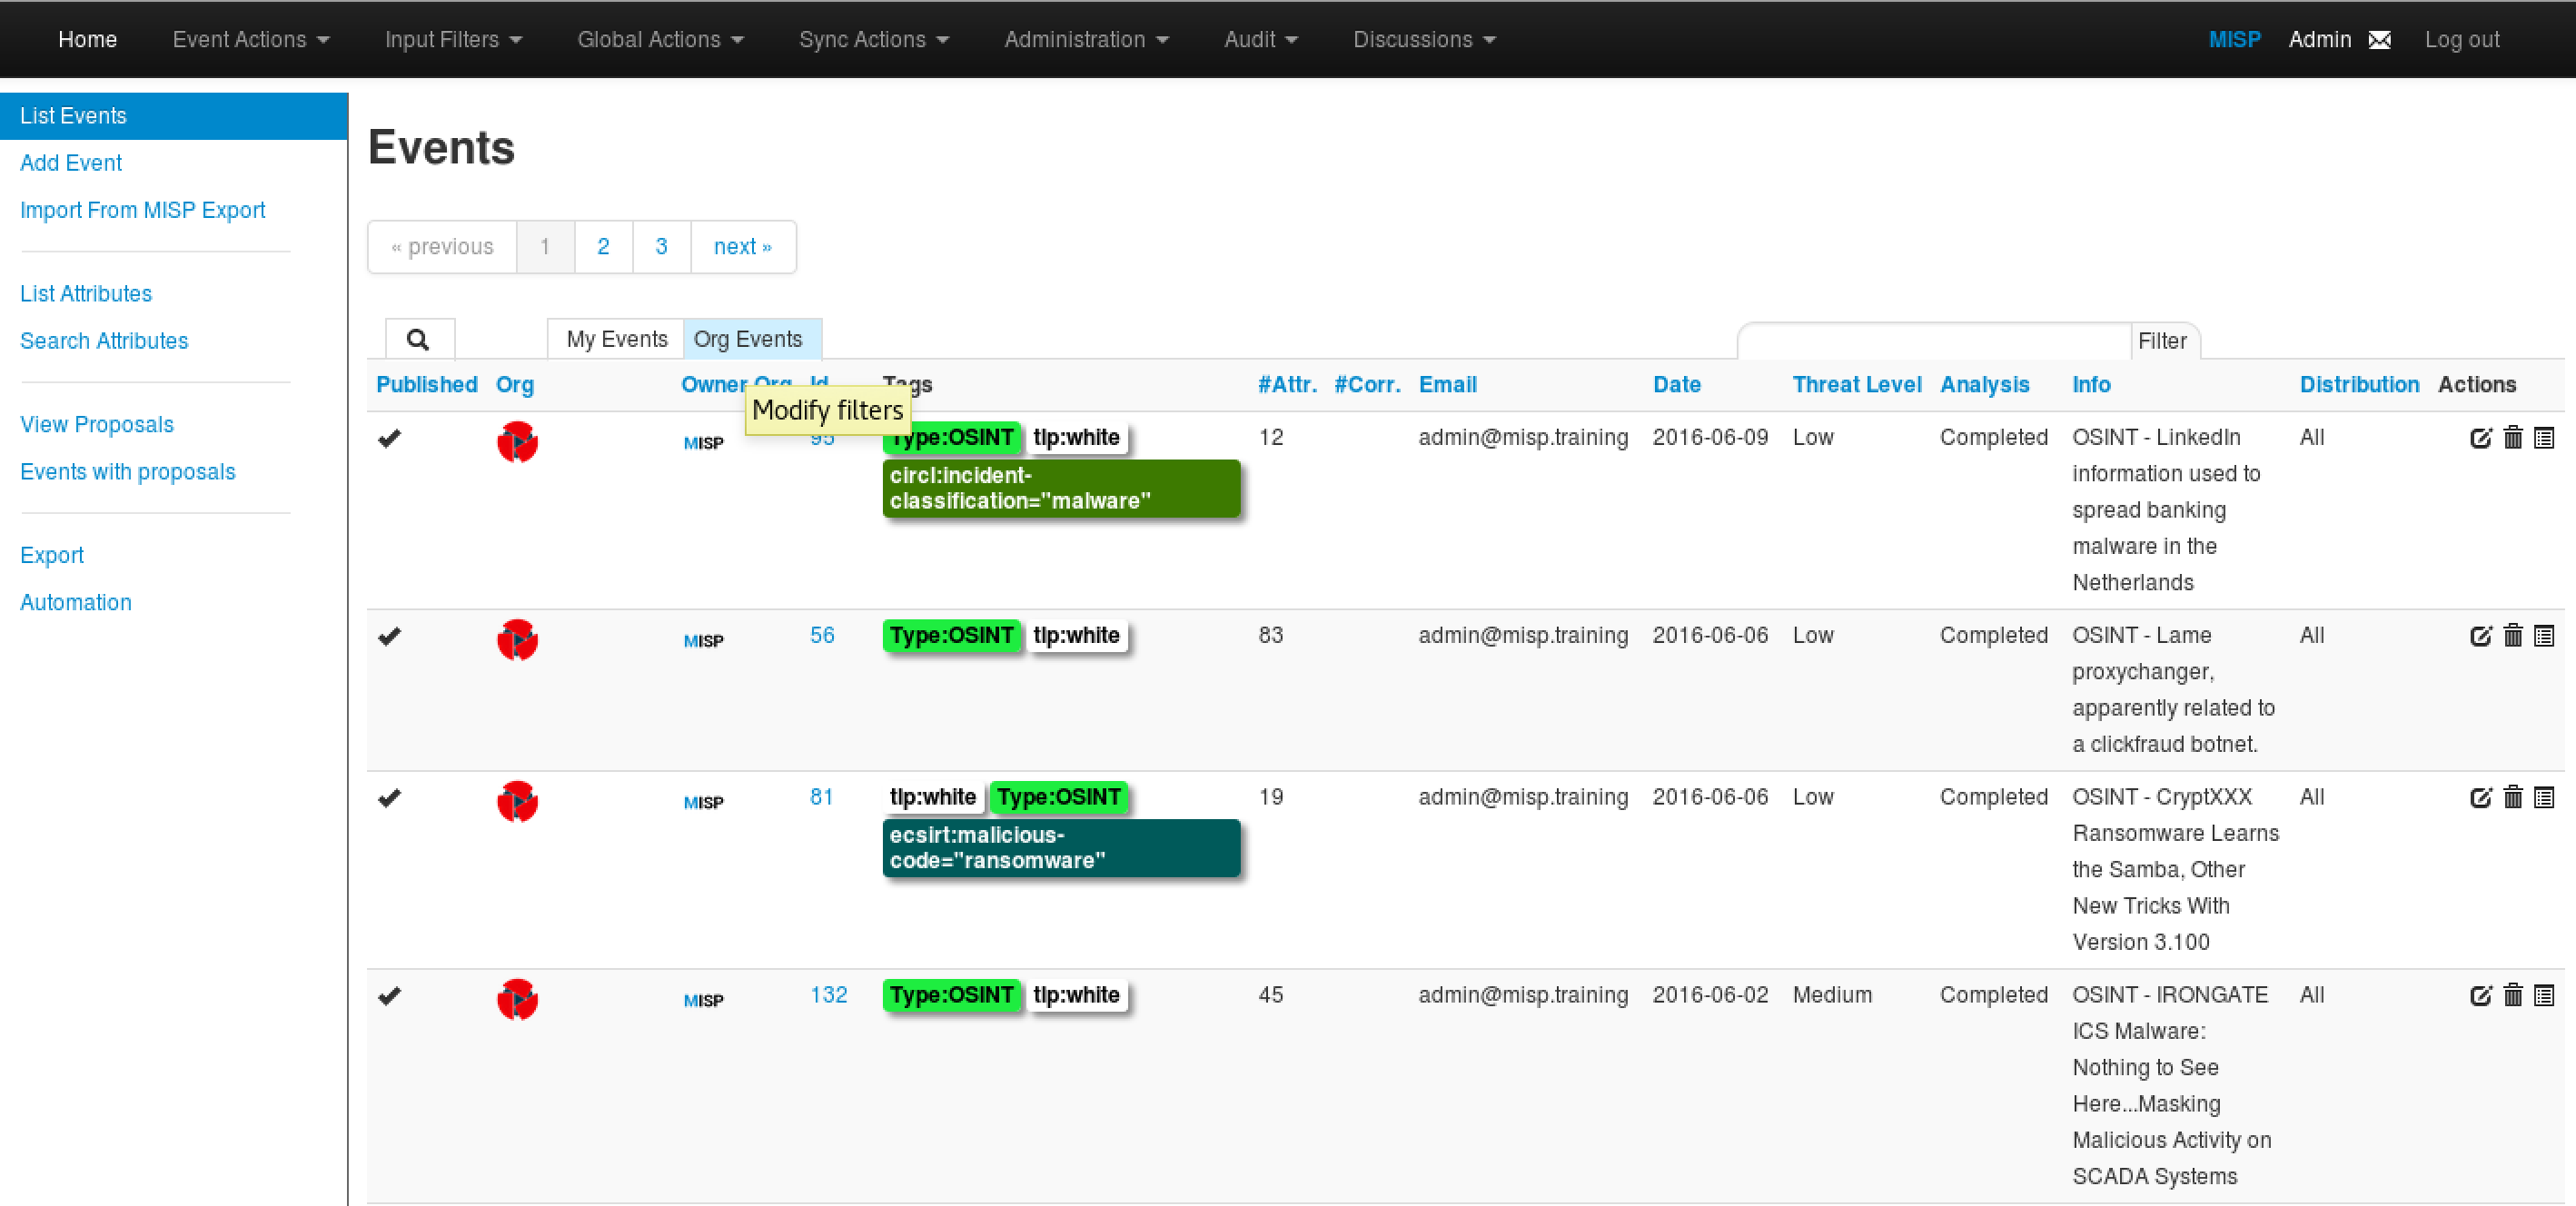
\includegraphics[scale=0.32]{res/webEvents}
		\caption{MISP : List of events}
		\label{webevents}
	\end{center}
\end{figure}


Then, by clicking on an event, we can get information on it \ref{webevent}:


\begin{figure}[!h]
	\begin{center}
		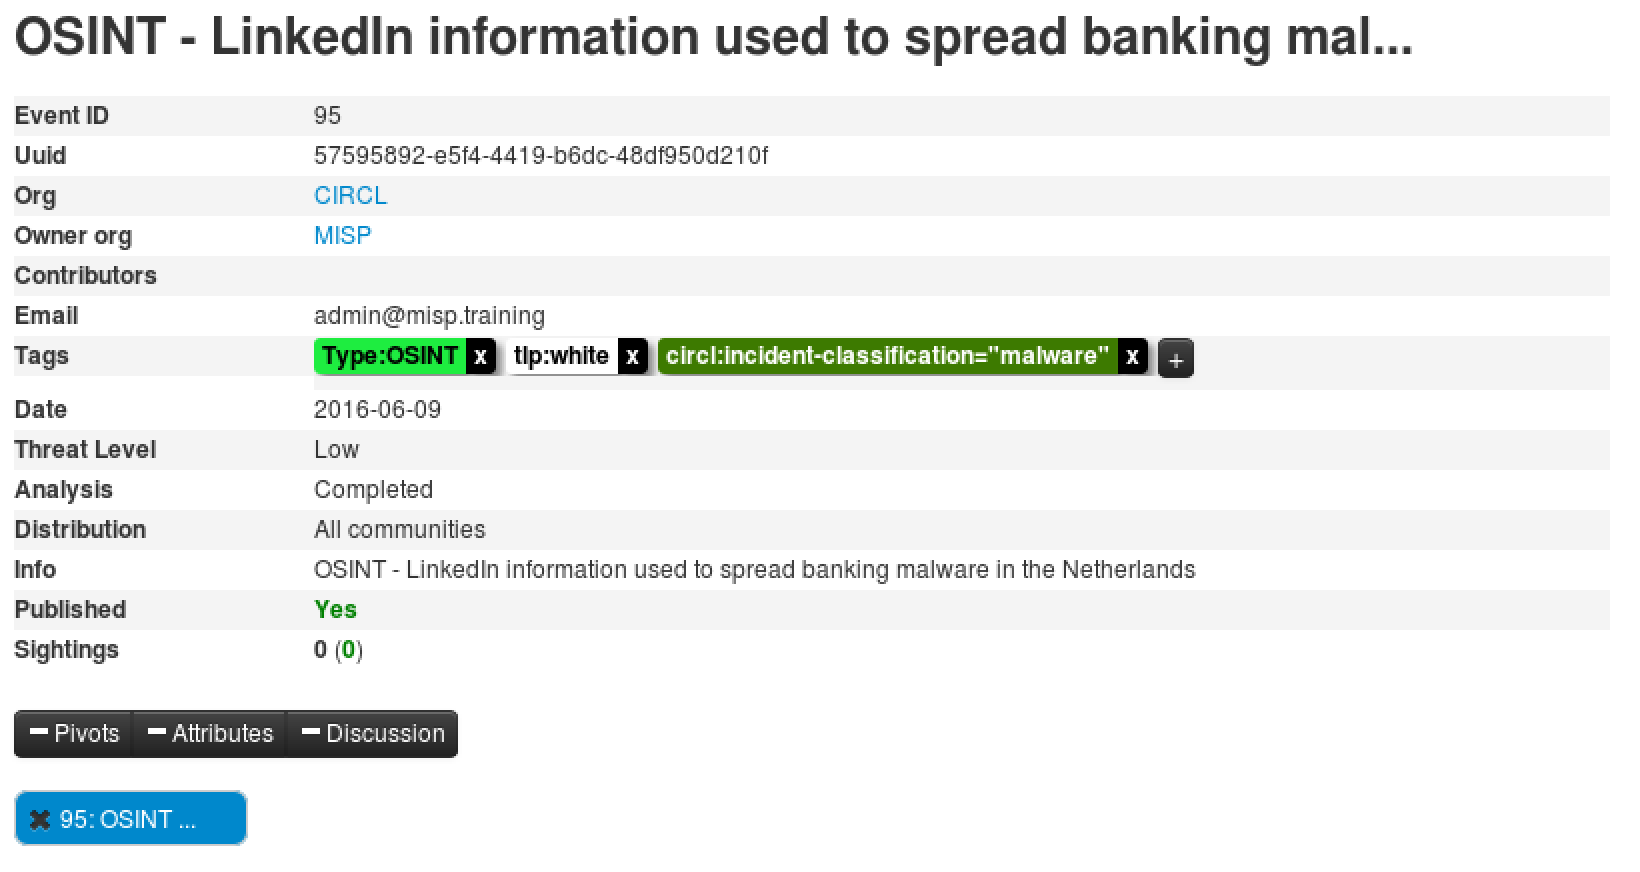
\includegraphics[scale=0.35]{res/webEvent}
		\caption{MISP : Specific information on the event}
		\label{webevent}
	\end{center}
\end{figure}


As well as the attribute list \ref{webattributes}:
\begin{figure}[!h]
	\begin{center}
		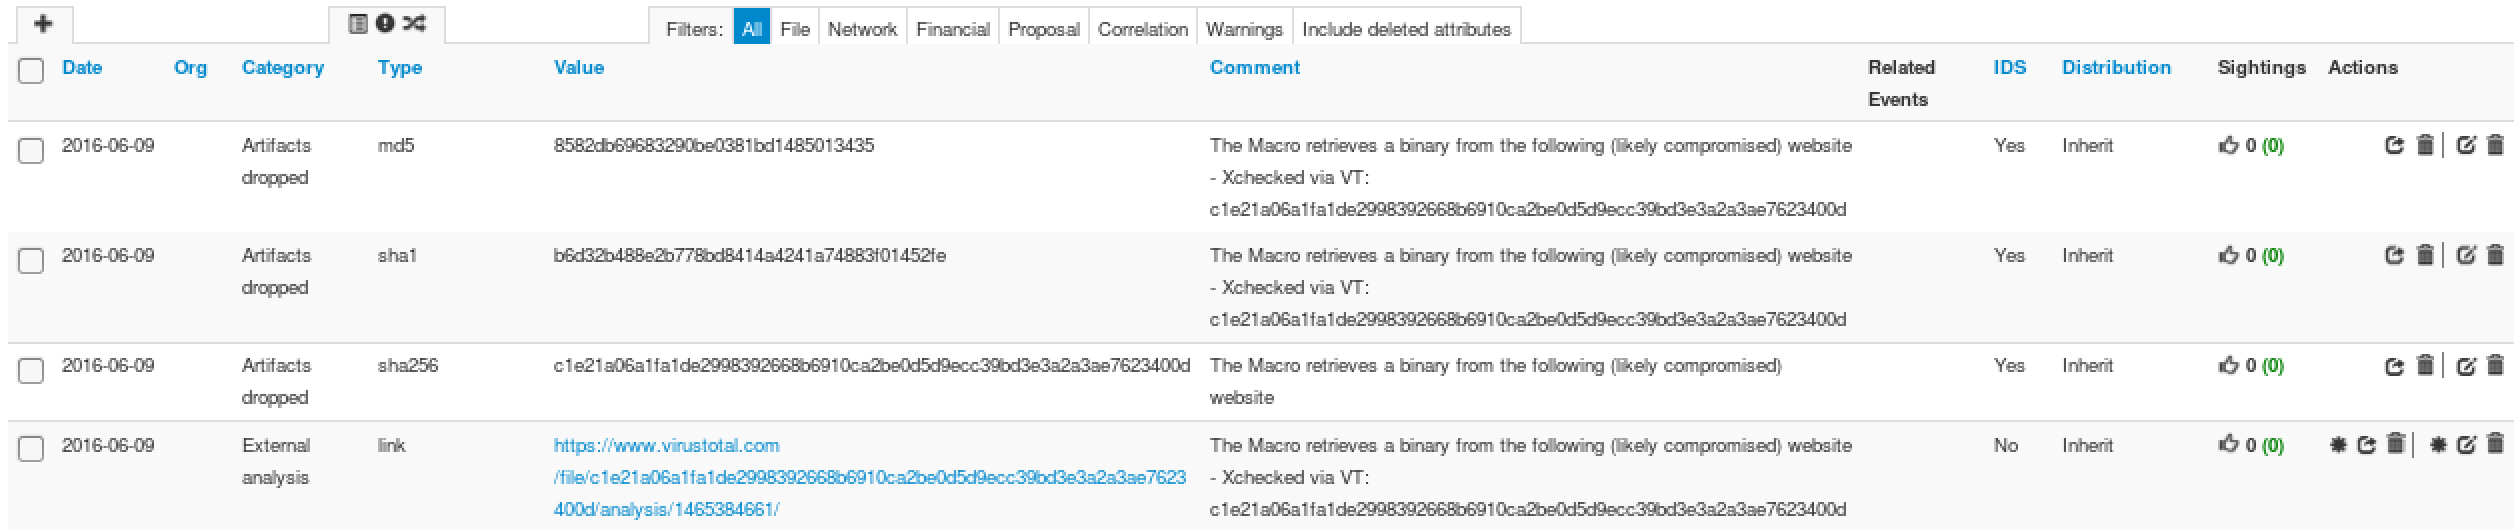
\includegraphics[scale=0.35]{res/webAttributes}
		\caption{MISP : Attributes of the event}
		\label{webattributes}
	\end{center}
\end{figure}

And the last thing that I want to show is one of the way of showing the correlations with other events and is called the correlation graph \ref{webcorrelation}:
\begin{figure}[!h]
	\begin{center}
		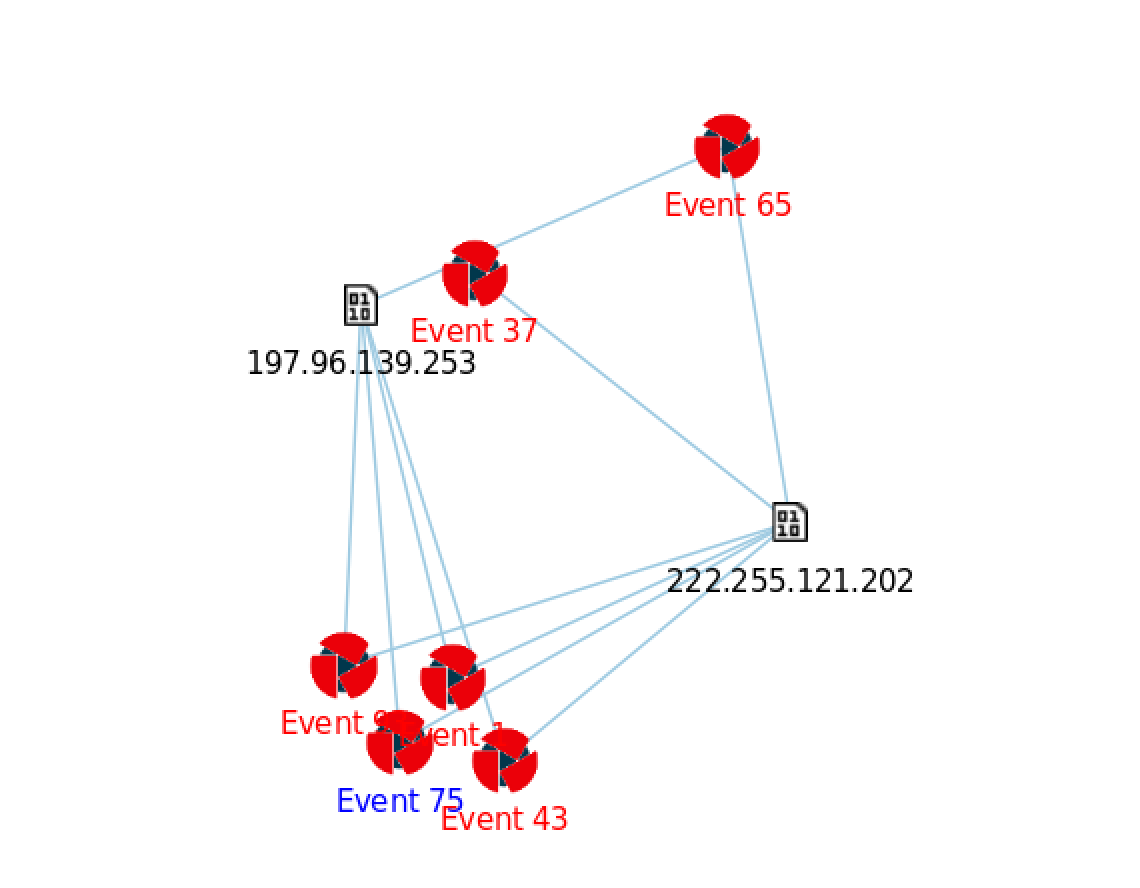
\includegraphics[scale=0.35]{res/webCorrelationGraph}
		\caption{MISP : Correlation graph for an event}
		\label{webcorrelation}
	\end{center}
\end{figure}



\chapter{Information Sharing State of the Art}

This chapter is aimed to give an overview of existing works in two domains, information sharing by itself and techniques used for privacy concerns.\\

\section{Information Sharing}
As usual, a good starting point is the already made state of the art about the subject, one really interesting was done by Gregory White and Keith Harison in \cite{white2017state} where they explain the evolution of the information sharing by comparing it with the evolutions of the USA laws and their impacts.\\
Even if the analysis is about the USA, I believe it is important to understand the origin of the concept. For an example, to know that the first attempt of sharing standardization was done just after the worm released by Robert Morris in 1988.\\
By analysing the impact of this worm, they rapidly realized that information sharing could have been a better and faster way to protect critical infrastructures. They also explain, in correlation with the two principal laws called the Presidential Decision Directive-63 in 1998 and the Executive Order 13636 in February 2013; how organization like Information Sharing and Analysis Organizations (ISAOs) where created with their four foundational objectives that can be summarized as:
\begin{itemize}
\item[$\bullet$] Each organization should be able to participate.
\item[$\bullet$] Development should be kept public.
\item[$\bullet$] Involvement should always be voluntary and should never be a requirement.
\item[$\bullet$] Take into account the need for confidentiality and privacy.
\end{itemize}
They also introduce the first sharing program developed by the Department of Homeland Security (DHS) which is the Cyber Information Sharing and Collaboration Program (CISCP).\\
With that, they introduce some standards like TAXII, STIX and CybOX explained in a few paragraphs. After that, they go through challenges that are facing the ISAOs. The major one is a privacy and confidentially concern, any information that an organization agrees to share with others, no matter who those others are need to be kept private and confidential and only released to individuals or organizations that have a right to have access based on the agreement that are signed by members of an ISAO. This concern is really interesting as this master thesis is really on trying to ensure that property without the need of trust. They also explained that privacy is that personal information about individuals within a member organization should remain private (in the context of information sharing).
While, confidentiality refers to information about organization that could lead to give others a competitive advantage.\\
In this article they were focus a lot on trust which is one of the most important property to ensure when dealing with a sharing group.\\
We cannot share confidential information if we do not trust the other party to keep it confidential and to respect privacy! \\

After that, a recent survey trying to compare the different vendors for threat information sharing was published in 2017 \cite{sauerwein2017threat}. The authors have conducted a systematic study of 22 threat intelligence sharing platforms and this article is a short sum up of their key findings I believe there is a lack of example to support their says, but it is still an interesting survey even if a detailed analyse of the 22 different tools would be really welcome.\\
On the other hand, their analysis of the different types, focuses, standards and licenses used by the different platforms bring a lot of information on what should be used in nowadays sharing platform.\\

I've introduced the name of some standards. They are really important as we cannot share if we cannot speak the same language. Thus these standards make possible threat sharing but also allow to make it automated. Besides that, when we decide to start in this subject. It is really too important to avoid making mistakes that perhaps have already been made. That is why some organizations like the National Institute of Standards and Technology (NIST) and the European Union Agency for Network and Information Security (ENISA) took care of publishing guidelines to help organizations to involve themselves in threat sharing.\\
In Europe, the Commission recognized that they have a role to play in making the information more secure. In order to do that, they wanted to create the first pan European Information Sharing and Alerting System (EISAS on which we can find a report on the implementation \cite{eisasRapport}).  They herefore have asked to ENISA to define the requirements. Afterwards, member states that weren't yet using information sharing were really interested by and asked ENISA to develop a good practise guide based on the observation of existing exchange. This gave this guide \cite{enisaguide2009} aimed to assist member states but also relevant stakeholders like organizations using communication network and information systems in setting up and running network security information exchange.\\
In this guide, they go through setting up information sharing but they also took care of explaining the advantages as well as identifying laws that could get in the way. This is really important as organizations need to ensure themselves not being recognized as a cartel or that sharing becomes a commercial advantage. They also focused on the trust that is needed, for them, it must be created thanks to regular face-to-face meetings and TLP must be used as well during these meetings.\\
Then, in 2016, NIST also published its guide \cite{johnson2014guide} that seems to me more complete and more mature. This publication is also more focused on organization than on States (unlike ENISA) and provides guidelines to improve cybersecurity operations and risk management activities through safe and effective information sharing practices.\\
For them, cyber threat information consist of IOCs, TTP (tactic, techniques and procedures), suggested actions to dectect, contain or prevent attacks and finally the findings from the analyses of incidents. \\
They go through different topics that are benefits and challenges encountered. How to establish and participate to sharing relations. Onces again, they draw attention on the importance of trust and to be compliant with legal and organizational requirements among other challenges.\\

On an other side, the paper written in February 2017 by Aziz Mohaisen et al. \cite{mohaisen2017rethinking} focus themselves on rethinking threat intelligence and to assess the risks. They argue by \cite{MalikThreat} that intelligence sharing is the only way to combat our growing skills gap in term of security. But they mostly claim that there are a lot of issues that needs to be explored in order to realize efficient and effective information sharing paradigms for actionable intelligence. They even go further by saying that understanding the risk of sharing as well as not sharing is absolutely needed for every organization.\\
Briefly, not sharing is a risk as we don't receive information that could avoid us to be compromised. But on the other hand, sharing information without proper restrictions may leak a significant amount of information about participant and their operation context and all that can be used by an attacker to learn their vulnerabilities.\\
One of the commonly proposed solution to that is to have a very limited sharing community only with highly trusted participants. But is it really what we need to do ? If the participant are not enough, we could also not succeed in gathering enough information.\\
But, if we have less trusted participant, we also need to understand to risk of leakage that could lead to both monetary and reputation loss. Taking all that into account, they propose new way of thinking for threat intelligence by defining models, communities and adversaries with their threat model.
They finally propose an architectural solutions as a way of assessing the quality of sharing.

\section{Existing Techniques}
Then, It is interesting to see existing techniques used in information sharing to ensure privacy and confidentiality in case where we do not want to rely on trust. This following paragraphs are used to discover what is used and what was used before in order to get ideas on what could be implemented.\\

The first idea is the simplest one and is about removing and hiding parts of the data. This technique is called data sanitization. Then there will be articles on secure two-parties (S2P) Computations.\\

One of the first article that presents some concerns about privacy in sharing security alert is \cite{lincoln2004privacy}.
More precisely, they were concerned about protecting site-private topology, proprietary content, client relationship and site defensive capabilities or vulnerabilities.\\
This was done in two steps, the first one, data sanitization, consist in removing confidential data and useless information: Don't take the risk revealing information to an attacker if this information is not needed by the user.\\
The second one is the correlation/aggregation work were alerts are linked together for analysis purpose.\\
 They have used three different categories of data coming from DShield ansd Symantec's DeepSight:
\begin{itemize}
\item Firewalls: They consider all "deny" as a possible attack
\item IDS: They remember logs of attacks that the IDS has found
\item Antivirus software
\end{itemize}

After removing all useless information, we can hash all confidential data. As the companies want to be insured of the confidentiality, they assume this job of directly hashing the data before sending them to the server.
This technique is quite well working if, the data has a certain size. But, on the other hand, it is not useful for IP addresses, if an attacker is targeting a company, it has to precompute only 256 or perhaps 65536 IP address hashes. Thus this is not brute force resistant.\\
For each alert, we have two different IPs, the source IP (ip\_src) and the destination IP (ip\_dest). We can classify all these IPs in two categories:
\begin{itemize}
	\item Internal IPs : IPs that belong to the company
	\item External IPs : IPs external to the company
\end{itemize}

The first category is, of course, the one that we need to protect and in order to do so, these IPs are hashed with a keyed hash function like HMAC. While the second type is only hashed by a simple hash algorithm like SHA-1.\\
The result is that we can compare all SHA-1 hashed IPs together while only companies can decrypt their own internal IP addresses.\\
An attacker cannot make the difference between an IP hashed by HMAC  or SHA-1. Thus, for attacking the dataset, he would need to try to crack all IPs as if they were SHA-1 fingerprints (For example with a TMTO attack). This, without forgetting that they receive millions of IPs, make it unfeasible for an attacker to bruteforce the whole dataset.\\
They are also using another set of protections like the randomized threshold for publication of an alert but it goes out of the scope of this work.\\ 
In sanitization, they also round all timestamps to the nearest minute in order to add some uncertainty.\\
The second step is the correlation, they spoke about historical trend analyses, source/target-based analyses and event-driven analyses. These analyses worth spending time on them but are not related to the specific subject of this work.\\

Then, \cite{xu2005privacy} was also working on confidential data sharing starting from the first article, but they came up with a new interesting idea, instead of hashing confidential data, why not generalizing it and doing probabilistic correlations.\\
\textbf{Guided alert sanitization with concept hierarchies:}\\
For example, if we have an IP 192.168.1.123/32, we can generalize it to 192.168.0.0/16.\\
The depth of the generalization is chosen thanks to the entropy or by the differential entropy technique explained in \cite{cover1991elements}.
\\
\textbf{Alert Correlation:}\\
They focused on defining similarity functions between sanitized attributes and building attack scenarios from sanitized attributes\\
They also used a technique to create probabilistic attack scenario which is a set of alerts put together to create a bigger attack.\\

These articles were looking at data obfuscation while still being able to create correlation analyses but, it is difficult to apply it in order to create a database of still usable data for prevention or detection as it looses information.
\\

I've explained some solutions that can be applied to IP addresses or file (like hashing them). But, what if we could do the same with all network packets and still getting some privacy!\\
That's the goal of \cite{parekh2006privacy}. Today, it's not enough to analyse IPs, URLs and so on. We need to go deeper in it, that's why they propose a technique based on the byte distribution of the packets.\\
They used PAYL and Anagram \cite{wang2006network} systems that they have created.\\

Sanitization is used to protect information by keeping privacy, but, as \cite{mohaisen2017rethinking} is referencing, there are other ways for sanitizing data. Some of them are k-anonymity \cite{sweeney2002k}, l-diversity \cite{machanavajjhala2007diversity} and the key privacy guarantee that has emerged is the differential privacy \cite{dwork2008differential}.\\
First, k-anonymity is an attempt to solve the problem of anonymizing a person-specific field structured data with formal guaranteed while still producing useful data. A dataset is said to have the k-anonymity property if the information for each person in the dataset cannot be distinguished from at least k-1 individuals. This is done by removing attributes or by generalization as seen earlier. This technique was unfortunately performing poorly for certain applications. Therefore l-diversity was an extension to it in order to handle some of the weakness of k-anonymity. It increases groups diversity for sensitive attributes in the anonymization mechanism.\improvement{Read cited articles instead of simple the first article to be sure of my understanding}\\

On the other side, we first focus on hiding data while sharing, an other point of view would be to be ready of sharing only if an benefit is guaranteed. For that, we make the hypothesis that the benefits that can bring such operations are directly linked to the amount of similar IOCs on each database.\\
Thus we need to find a way to get the intersection or the cardinality of the intersection of these two database without leaking any other information. Fortunately for us, there exists algorithms for that called Secure two-party computation.\\
With these metrics, we therefore can make a thoughtful decision of sharing.\\
The paper written by Freudiger et al.\cite{freudiger2015controlled} focused on this problem by working on a DShield dataset. They've experimented some strategies to know if it could be useful to share or not with another organization. And then, they also experimented to share the whole dataset of the company, only the data set linked to the intersection other dataset or only, the intersection (just to get a rough idea of what they have in common ... ).\\
Their conclusion were intuitively expected but still interesting :
\begin{itemize}
\item More information we get on an attacker, the better the prediction are.
\item The chosen collaboration strategy has a really big impact (some of the strategies are really useless).
\item Collaboration with companies improves not only the true positive rate (called predictions accuracy in the article) but also removes a lot of false positive.
\item Sharing only about common attackers is almost as useful as sharing everything.
\end{itemize}

This king of secure two-party computations are used a lot and is also used in some articles for multi-party private matching. And other important way of calling it in health report is Privacy-Preserving Record linkage (PPRL)
\info{I'm reading articles on it, it is really nice! I will see if it ll come in further work or here or if I have time to implement something more !}

Now that we see more concretely what is information sharing, a good question is to understand how it is used in nowadays system. In MISP, it has mainly two utilities. The first one is to be able to gather the information of more team that could work on similar incidents and make them collaborate on their searches.\\
The second one is about directly protecting computer systems by using the information the user has access to create rules for an Intrusion Detection System (IDS) like Snort, Suricata or Bro. These IDS rules can be directly generated inside MISP. The contribution of this master thesis would be to be able to create rules for events that the user could not have direct access as he could not directly get back informations from the rule.\\
These rules also work in Intrusion Prevention System (IPS) but it is still important to consider the IDS version with the analyse of network logs in the system. This is useful as sometimes the information of an attack is known after the attack and if it went undetected perhaps the attacker is still on the system and we need to know it as soon as possible.\\
Today the estimation is that the mean time an attacker stay on a system before being detected is of about 200 days which can have dramatic financial consequences but also mostly on the clients' trust (Considered as the biggest cost by the Ponemon Institute).



\section{Standards}
As we want organizations to share threat information, we need them to "speak the same language" or more formally, to use the same standards.\\
For that, we can categorize the standards into four categories (standards list can be found in \cite{AwesomeTreat, mohaisen2017rethinking}):
\begin{enumerate}
\item Enumerations
\item Scoring Systems
\item Languages (CybOX, STIX, MISP-core format)
\item Transport (TAXII)
\end{enumerate}

I will only focus on the four cited before. From these articles \cite{fransen2015cyber, sauerwein2017threat}, we can read that the most promising standards for a threat sharing intelligence sharing infrastructure are CybOX, STIX and TAXII. They have been developed under coordination of the MITRE Corporation and have very strong momentum in adoption by industry leaders and threat intelligence communities such as the Financial Services - Information Sharing and Analysis Center (FS-ISAC).\\
The  Structured Threat Information eXpression (STIX) \cite{barnum2012standardizing} provides a language to represent cyber threat information in a structured manner and it provides a structure to express a wide set of contextual information regarding threats in addition of the IOCs. The complete list is :

\begin{itemize}
\item[$\bullet$] Cyber Observables
\item[$\bullet$] Indicators
\item[$\bullet$] Incidents
\item[$\bullet$] Adversary Tactics, Techniques, and Procedures (including attack patterns, malware, exploits, kill
chains, tools, infrastructure, victim targeting, etc.)
\item[$\bullet$] Exploit Targets (e.g., vulnerabilities, weaknesses or configurations)
\item[$\bullet$] Courses of Action (e.g., incident response or vulnerability/weakness remedies or mitigations)
\item[$\bullet$] Cyber Attack Campaigns
\item[$\bullet$] Cyber Threat Actors
\end{itemize}

 One of its real advantage is taht it tries to stay as "human-readable as possible". The complete STIX structure is deeply explained in the ninth chapter of \cite{barnum2012standardizing}.\\
 For expressing the observable, STIX is using the Cyber Observable eXpression (CybOX)\cite{barnum2012cybox} that allows to state the specification of events or stateful properties. At first, CybOX was developed independently but is now integrated into Version 2.0 of STIX. It is a Structured language for cyber observables.\\
Then, we need a standardized transport mechanism and for that, we have the Trusted Automated eXchange of Indicator of Information (TAXII) \cite{connolly2014trusted, TAXIIProjectWeb} which is community effort to standardize the trusted, automated exchange of cyber threat information. It defines a set of services and message exchanges that, when implemented, enable sharing of actionable cyber threat information across organization and product/service boundaries for the detection, prevention, and mitigation of cyber threats..\\
TAXII is defined around sharing models. There exist three of them:
\begin{itemize}
\item \textbf{Hub and Spoke}  is a sharing model where one organization functions as the central clearinghouse for information, or hub, coordinating information exchange between partner organizations, or spokes. Spokes can produce and/or consume information from the Hub.\\
\centering
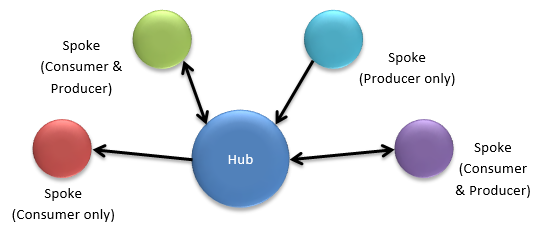
\includegraphics[scale=0.5]{res/hub-and-spoke}
\item \textbf{Source/Subscribers} is a sharing model where one organization functions as the single source of information and sends that information to subscribers.\\
\centering
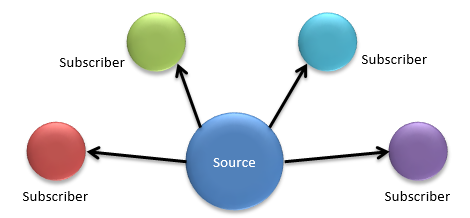
\includegraphics[scale=0.5]{res/source-subscriber}
\item \textbf{Peer to Peer}  is a sharing model where two or more organizations share information directly with one another. A Peer to Peer sharing model may be ad-hoc, where information exchange is not coordinated ahead of time and is done on an as-needed basis, may be well defined with legal agreements and established procedures, or somewhere in the middle.\\
\centering
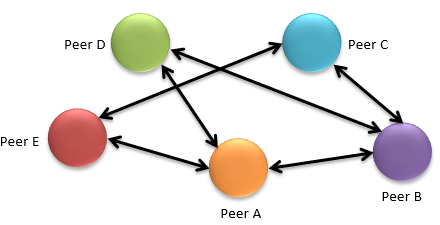
\includegraphics[scale=0.5]{res/peer-to-peer}
\end{itemize}


On the other hand, in the MISP project, they decided to support more attribute types and to have an easier model to use. Therefore, A. Dulaunoy and A. Iklody describe an alternative, the MISP core format, in the second version of the draft\cite{MispDraft} while still allowing to directly export data into the STIX format in the web interface. On the other hand, they are using the Hub and Spoke TAXII model for transportation as explained in the introduction.

\section{Contextualization}
When I started the master thesis, my knowledge about threat information sharing was clearly none. I had to look up for articles and information where I was able to find some. I've finally chosen some articles and some points that I found interesting to share in order to understand the different steps I followed and the different ideas on which I thought about.\\
Also, I've spoken about MISP as it is the platform I'm interesting in but there is an available really good awesome list \cite{AwesomeTreat} available where a bunch of existing standards, tools and techniques available in this domain are listed (Unfortunately I found it only at the end of the master thesis).\\
But in order to come back to MISP. The main advantages compared to the proprietary solutions are that :
\begin{itemize}
\item[$\bullet$] Transparency in term of code and of the contributor.
\item[$\bullet$] Quantity and diversity of connected entities
\item[$\bullet$] The price and the non-existence of entrance barriers\info{Any additional are welcome}
\end{itemize}

On the other hands, there exist also other kind of platforms like DShield but they are sharing the whole bench of indicators and deals with a lot of data while MISP is more interested in events and in the analyses of what is going on.\\

In the state of the art, I've also spoken about attack scenarios and cardinality of intersection to evaluate the benefit of sharing before doing it. These kind of techniques are not yet implemented in MISP but could appear one day.\\

Back on the sharing problem have a data set of malicious data, IOCs, events coming from MISP and we want to share them in a privacy-preserving way and moreover, we want to get rid of this needed trust in sharing.
It would be really nice, computer specialists would be able to check on computers to discover infections, problems and moreover learn how to fix it thanks to the previous analyses contained in MISP. The problem is that some information are confidential and we need to have some confidentiality concerns while sharing. \\


Then, it was really useful to see these existing techniques but it unfortunately does not mean that it could solve all of our problems. They had other purposes when designing their solutions and it can lead to some disadvantage in what we are attempting to do.\\
Sanitization is a good example as it is really useful for the existing implementation but in this case, it would modify data up to make them unusable for every one.\\
Other sharing strategy needs server always up which is not interesting either so we still need to find a way of sharing only if the user has really knowledge of the event and can share information on it as well, or is really infected by and need help that could be given by the information.\\


\section{Misp-Worbench - hashstore}

MISP workbench\footnote{https://github.com/MISP/misp-workbench} is a set of tools to export data out of the MISP MySQL database and use and abuse them outside of this platform.\\

CIRCL has already implemented a privacy aware tool called hashstore and implemented in redis\footnote{http://redis.io}. This is working by creating a dataset of all hashed IOCs. And then by the use of the redis server, we can use a redis client to request data.\\
Like that, if you want an information on a particular IOC, you need to already know it to be able to take its value's fingerprint and make the request.\\
On the other hand, coming back on the small data problem, if we consider an attacker that want to try every possible IPs, for IPv4 it represents 4.228.250.625 different IPs that needs to be tested. Even if it is a lot it is still feasible as redis is really fast. Moreover, not all IPv4 need to be tested, for an example we can avoid private subnet like 10.0.0.0/8, 172.16.0.0/12, 192.168.0.0/16 which already represent 17.891.328 addresses.


\section{Limitation: What could be expected}

As discussed with the risk, there are a lot of privacy concerns about sharing data. And therefore, a lot of separate techniques. But there is an additional important problem that needs to be taken care of. For example, one of the solution for preserving privacy is simply hashing the data. For big sized data, it's not feasible to brute force it but, for IP addresses, since in general, there are only 256 or 65536 different IP addresses in the range of IPs of a specific company, we could create a table with all possible hashes and test them all!\\

But still, the idea that a common user have access to data while an attacker, which is a specialist, cannot seems infeasible in a lot of cases. The attacker always ends with the data but, if he takes 1 second, 1 day, 1 week, 3 months or years is different because, we can then think about how long a data is valid? \\

These questions are important as we want to share the data in a way that a user could get the complete database on its computer and make requests on it without needing an internet access.\\
We thus now that brute force attack on suck system are unnoticeable and also that it is intrinsically impossible to fully hide small IOCs while still allowing a subscriber to evaluate the rule. \\

The solution I'm looking for will thus approach the real solution but we already know that it cannot be perfect.

\chapter{Standards Ideas}

Now that the subject seems clearer, there are a lot of different possibilities that could be explored. This chapter will be the opportunity to dwell on some of them in order to look for their strong points as well as their weaknesses.

\section{Bloom Filters}
Bloom filter is a space efficient probabilistic data structure  used to efficiently test the membership of specific values.\\
It has an enormous advantage which is to be able to test for membership without requiring to store the complete set of member data. On the other hand, even if this data structure never forgets a member, it can falsely believe in the membership of a data even not related to it. The rate to which a data is wrongly recognized is called the false positive rate and will be explored later on.\\
This small example of a small dataset of small data already shows the memory advantage: the data set of all the students' name and surname at Harvard. Taking the hypothesis that each name and surname has approximately 6 characters and that there are about 20 000 students. The dataset should use 20 000 * 6 * 2 * 8 (=1920 000) bits while a 1\% false positive bloom filter could be only around 20 000 * 10 bits which is already more than 9 times smaller.\\

\subsection{Data Structure}
A bloom filter is a m bits array (fig. \ref{bloom-1}) all set to 0 at the starting point. Besides that, there are also k independent hash functions. 

\begin{figure}[h!]
	\begin{center}
		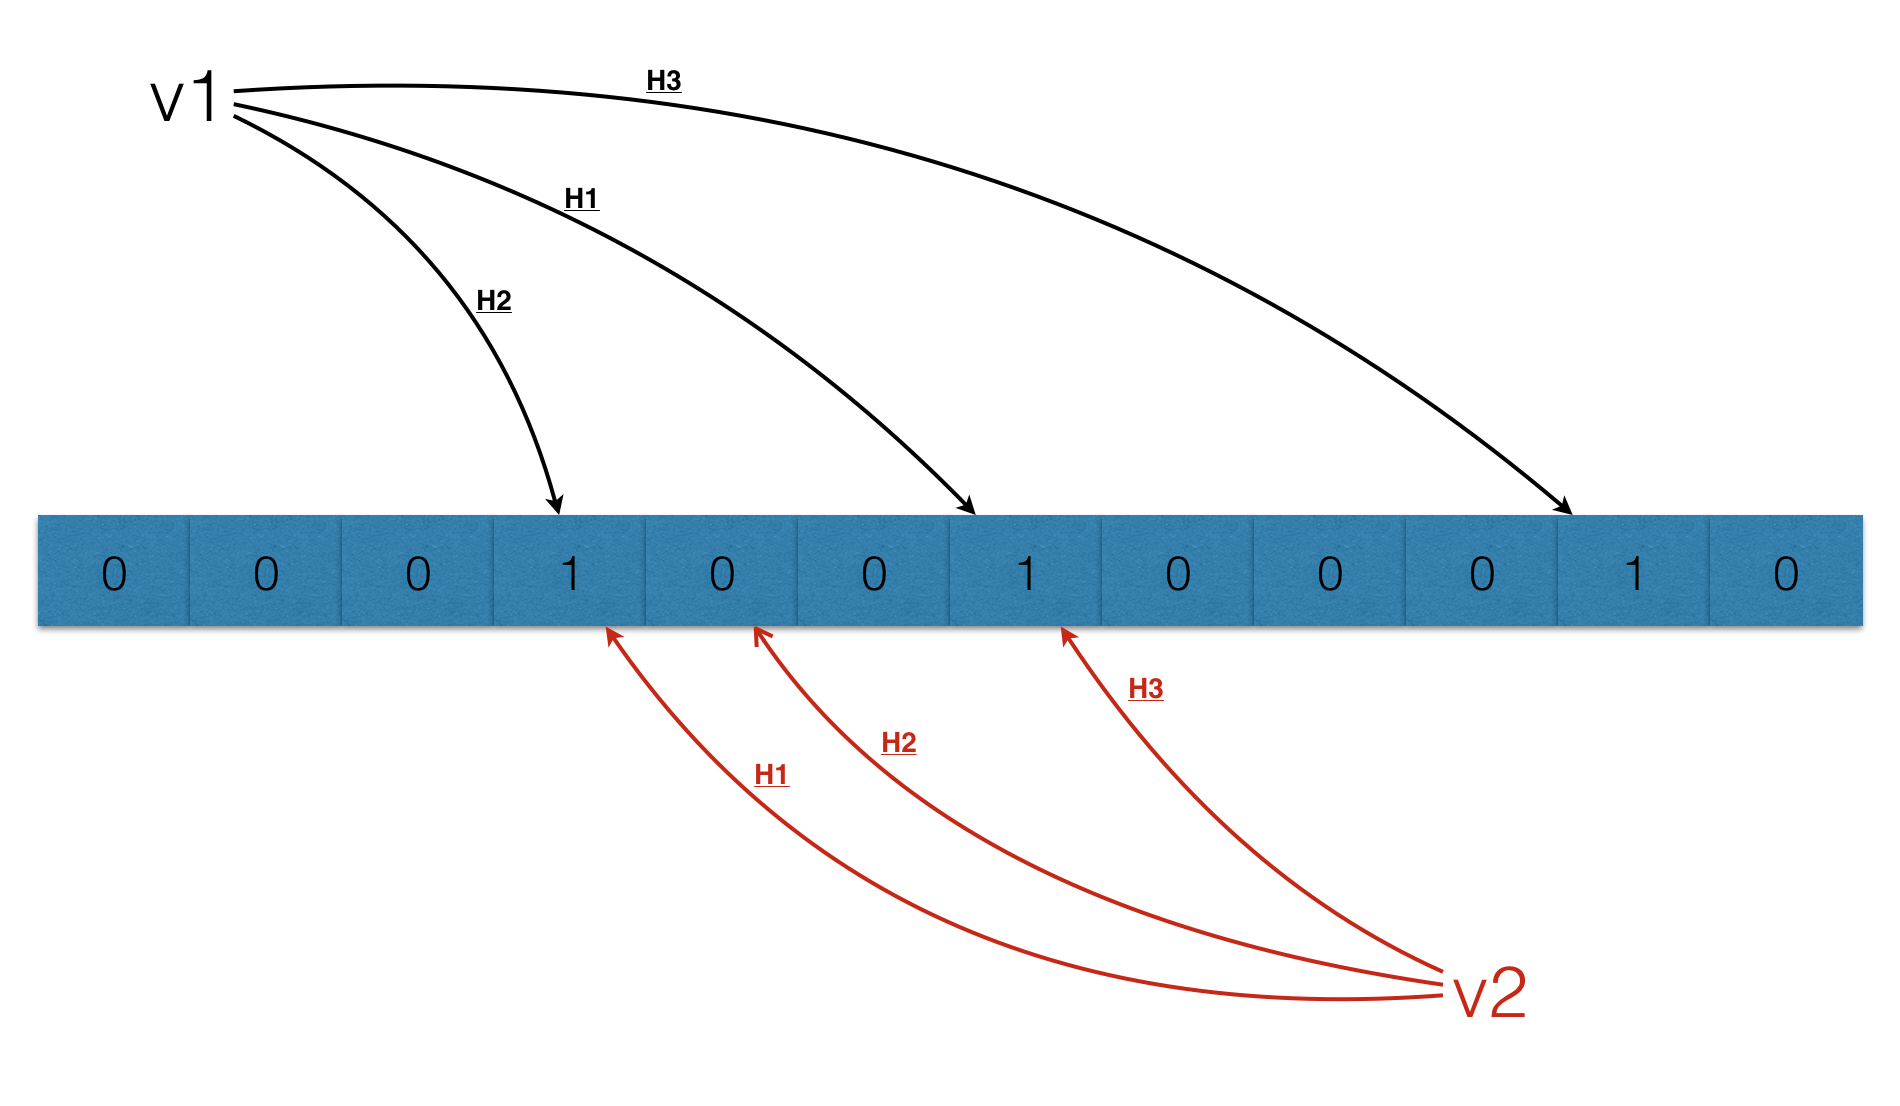
\includegraphics[scale=0.3]{res/bloom-1}
		\caption{Structure of a bloom filter with m=12 and k=3}
		\label{bloom-1}
	\end{center}
\end{figure}

To add the value v1, each hash function gives a fingerprint of the value which is considered as an index in the array where the value needs to be set to 1. In the opposite, if we want to test a value for membership, we have to check all indexes given by the hash functions. As we can see on figure \ref{bloom-1}, v1 is in the set while v2 is not.

\subsection{False Positive Rate}

Bloom filter is a probabilistic data structure as when we are checking for a value, either the value is \textbf{not} in the set or is \textbf{perhaps} in the set. \\
In the latest case, this is due to false positive where all the k hash functions gives indexes already set to 1 while the element should not be in the set.\\
An example can be seen on figure \ref{bloom-2} where v3 do not belong to the set.

\begin{figure}[h!]
	\begin{center}
		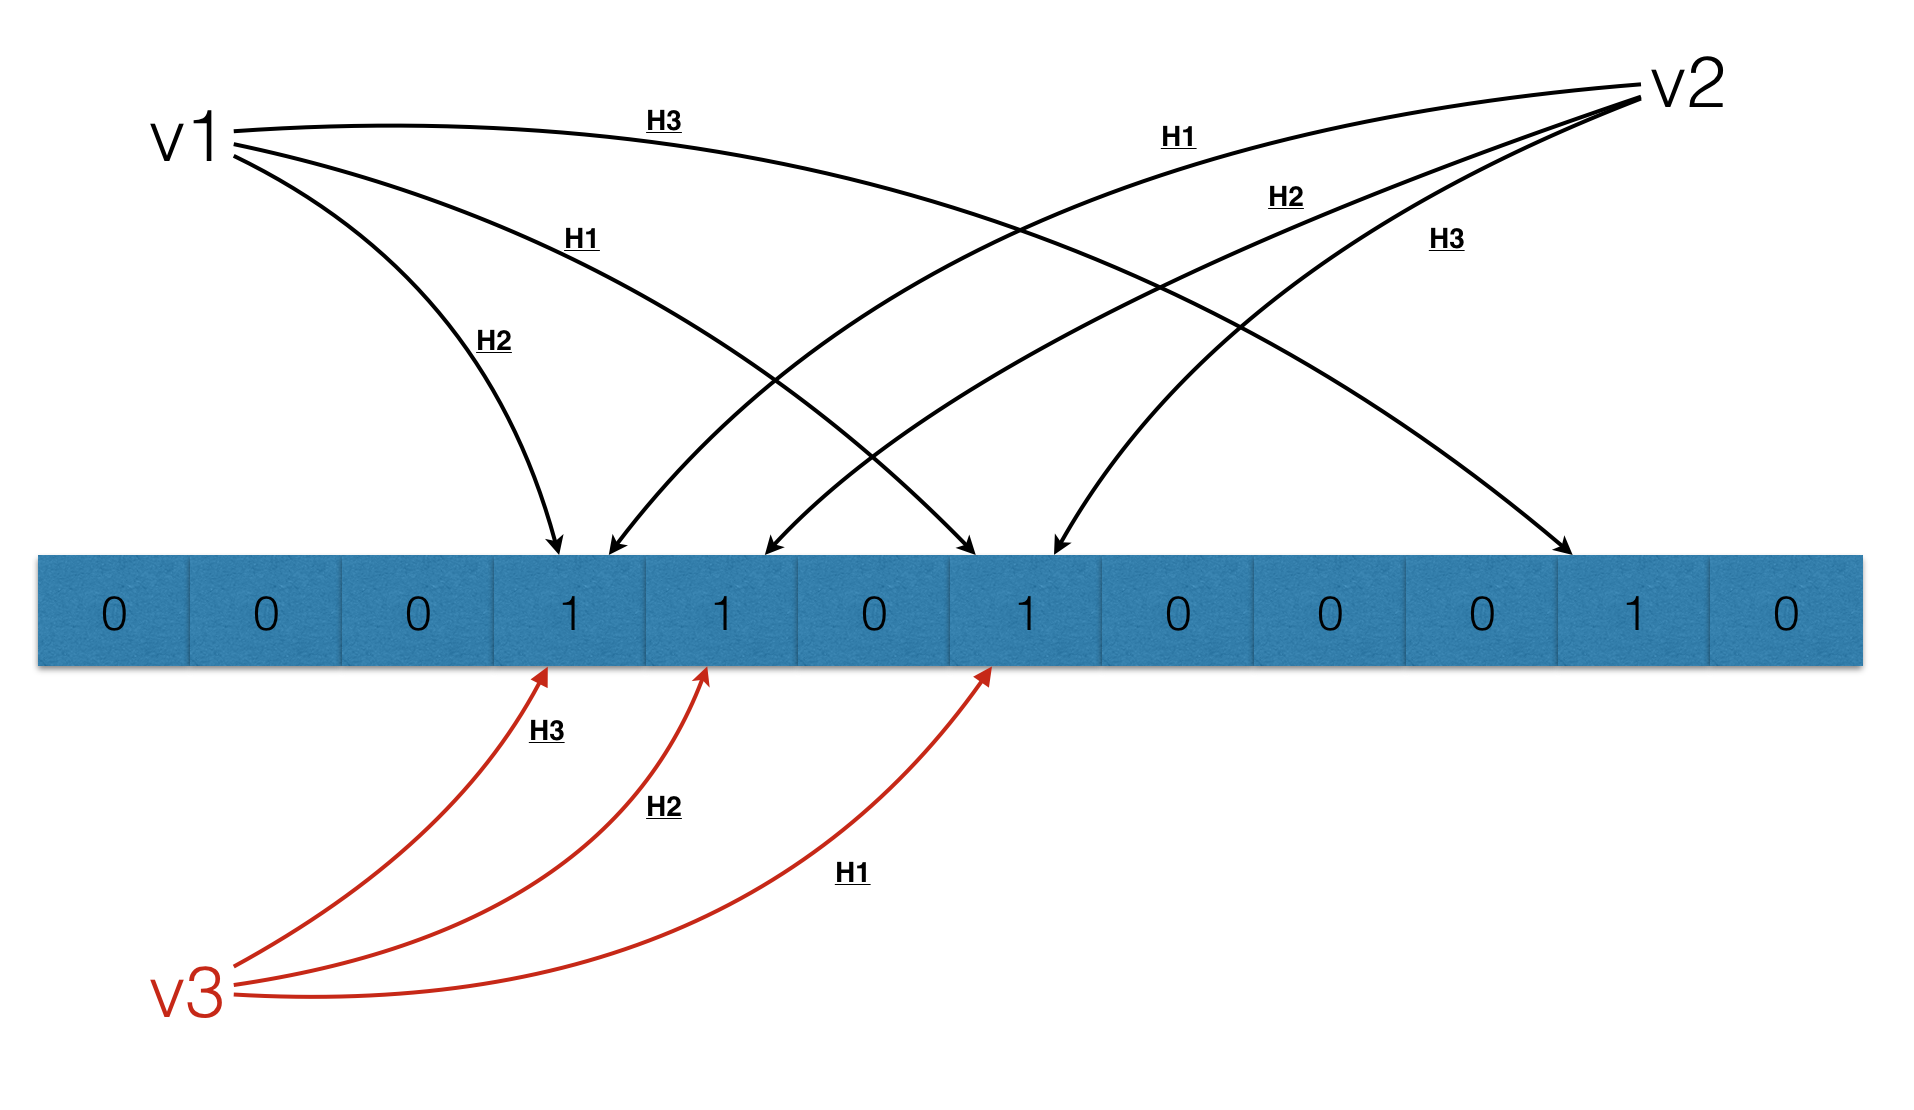
\includegraphics[scale=0.3]{res/bloom-2}
		\caption{False positive v3 in a bloom filter with m=12 and k=3}
		\label{bloom-2}
	\end{center}
\end{figure}

\subsection{Control the False Positive Rate}
If we check for a value in a bloom filter, at the end, we only know if it is not in the set or a probability to be in the set. Playing with this probability could be interesting for hiding some information and can be a really important feature for privacy and confidentiality.\\
This is why it could be useful to get more information on the false positive rate and how we could use it.\\

If n is the number of element inside the data structure we can approximate\footnote{https://en.wikipedia.org/wiki/Bloom\_filter} the false positive rate by $(1-e^{\frac{-kn}{m}})^k$ but a more useful way is to define k in function of the willing rate for the false positive. In this case, we can notice that k is independent of the number of element inside the set while on the opposite, it is m who needs to be changed in function of the number of values n:
$$m = - \frac{m\ \ln(p)}{\ln(2)^2}$$
$$k = - \frac{\ln(p)}{\ln(2)}$$
(These are approximations)

\subsection{Information Leaked by Bloom Filters}
It could seems useless but nevertheless it could have huge impacts. If we create bloom filter and we ensure a false positive rate, with the size of the array (m), the number of hash functions (k) and the number of bit set to 1(X). An attacker could approximate the number of values in a bloom filter like shown by Swamidass et al. \cite{swamidass2007mathematical}:
$$n* = - \frac{m}{k} \ln\left[1 - \frac{X}{m}\right] $$

This does not bring a lot of information and the number of elements in the set is leaked as well in the final solution but it is important to have a knowledge of that while implementing a system based on those solutions.

\subsection{Is this a complete solution to the problem?}
It is not enough alone as we not only need to test element for membership but we also need to get back information on it.\\
But it is still an interesting solution and could have great benefits once twinned with a later explained implementation .

\section{Machine Learning}

Machine learning is \textbf{the} actual technology for security. A system that could evolve and learn by itself. No need for updates! \\
Early in April, "Beyond the blacklists: Detecting malicious URL through machine learning" showed at the Black Hat Asia conferences that it can work.\\
They focused on URL lexical feature like the URL length, vocabulary, path, hostname, parameters, HTTP headers (in average, there are less fields with malicious connections) and they manage to get a 84\% detection rate on about 750K malicious URLs which is really promising.\\

Machine learning is thus a really promising tool in this domain but, the idea here would be to use it completely differently. We don't want it to continuously learn but we want an algorithm to learn a specific data set.\\
Then the control of false negative and positive would be done via overfitting.\\
In this particular case, overfitting is what is needed as we are not interested in inference but just in recognizing the elements' membership.\\

This technique could be interesting to keep more control on the privacy and confidentiality, an attacker would learn even less things than with a bloom filter.\\
For the size, a model can also fit with less memory than remembering the whole set but will differ in each algorithm.\\
So the base concept representation (BCR) of this technique on different example could bring a lot of information on the usability of this technique. But it could be difficult to tune and would have the same disadvantage as the bloom filter which is that it only decides membership and cannot give useful data back to the user. One last important thing to be aware is that some kind of models could leak information inside them for someone really understanding the system. (Ex clear decisions for a decision tree)\\

This technique has the advantage of bringing more data protection due to the false negative rate but it also looses an important characteristic as it could be bad to know an attack IOCs but do not detect it because of that rate.

\section{Secure Multi-Party Computation}
Each organization possesses its IOC database and is not ready to share all their information. But, once again, if it could help an other organization to solve its problem, they agree on sharing only these information.\\
That is where Secure Multi-Party Computation could play a role as there are techniques to find the intersections of 2 datasets. This is also called private matching \cite{agrawal2003information, li2005private}.\\

This technique has only a big disadvantage which is heavy computations on both sides. But still, it could be very useful to share information between MISP instances.

\section{Proof of Work Database}
This idea is to slow down brute force attack thanks to proof of work. Even if this idea is one step closer to the final implementation, it is still different by the need of a server to communicate with for each requests.\\

Here, we want to keep a database, we don't want any false positive nor false negative. But by doing that, we make our database available to brute force attacks.\\
We just need to add a new wall of time consuming computation between the user and the dataset for the requests.\\

A possible implementation could be with a random key chosen by the database server. This key could be regenerated with a small period and also every 1000 thousands requests.\\
On the other hand, the client should brute force this small key each time it has changed. This slows down brute force attacks while still be useful for a user that is doing less than 1000 requests to test its system.

For example, a possible request message for an ip could be : hash(IP)||hash(IP||key)\\

The idea is interesting even if it is still not bullet proof against brute force attack. It also need a server to respond at each request.

\section{Conclusion}
I've explained some basic ideas that could lead to different implementations, lot of work are done especially on private multi-party matching that could lead to the best option if requests are rare or, for example if it is used to periodically compare and synchronize data related to the same events between MISP instances.\\
Nearly all solutions still needs a server that we would like to get rid of (After the data had been generated) and for that, a machine learning model or bloom filters are the right track but there is still a lack as we do not get back information. That is why the final implemented solution will find something similar to proof of work  to slow down the attack and the bloom filter to increase the system speed.



\chapter{Implementation}
I've explained ideas in the previous chapter, some of these could be implemented. But a nice article \cite{van2016private} was published in the few first months of my work and they had found a technique that could also work here as their goal was similar one: allow parties to share information without the need to immediately reveal private information.\\
Their implementation was for bro, here I will make an implementation working with MISP and improve its matching properties and the modularity of the code. \\
By modularity, I mean that I want to be able to add "cryptographic modules" in order to test different techniques with the same code.\\
In this chapter, I will first explain their article, then the modifications I've made with some improvements.\\
A discussion on the libraries and tools will follow before benchmarking tests and discussions on the implementation in the next chapters.

\section{Private Sharing of IOCs and Sightings \cite{van2016private}}
This paper consider a cryptographic approach to hide the details of an indicator of compromise. They consider two different phases, sharing these IOCs and privately reporting the sightings of IOCs.\\

Reporting the sightings is important for monitoring the events and attributes in MISP.\\ 
Moreover MISP is now able to remember a sightings number per attribute but their technique seems difficult to implement in MISP for a standard subscriber as we should go through each attributes for each instances and each reporters while being online periodically (not practical at all). I've got some other ideas but I finally only focused myself on the sharing part as I would have not enough time.\\ 
But still, It could be the most important and really useful further work to do.\\

They also started by warning the reader that using these cryptographic function is better than not using them at all but it is not a miracle technique as it is theoretically impossible to hide the IOC’s content in the used context (Subscribers receive the data to check on its system).\\
Additionally, it has a performance cost but in my beliefs, it is well worth it.\\ Their implementation is in the source-subscriber TAXII sharing model but it can nevertheless fit with our model.\\
First, they define an IOC as propositional formula where the propositional variables are defined over features or observables like Internet Protocol (IP) or fingerprints of malicious program (but it could be any categories of MISP). They also claim that every IOC can be expressed in the Disjunction Normal Form (DNF) without any negation (e.g. destIP= 198.51.100.43 $\land$ destPort = 80).\\
Hereandafter the values of the rules generated are considered as the concatenation of all values of the IOCs contained in a rule : IPv4$||$port\_number. It has two advantages, the first is to represent all linked values directly together and then increasing the size and the number of element hashed increases the difficulty for an attacker to perform a bruteforce attack or to precompute all possible hashes.\\

\begin{figure}[h!]
\begin{center}
	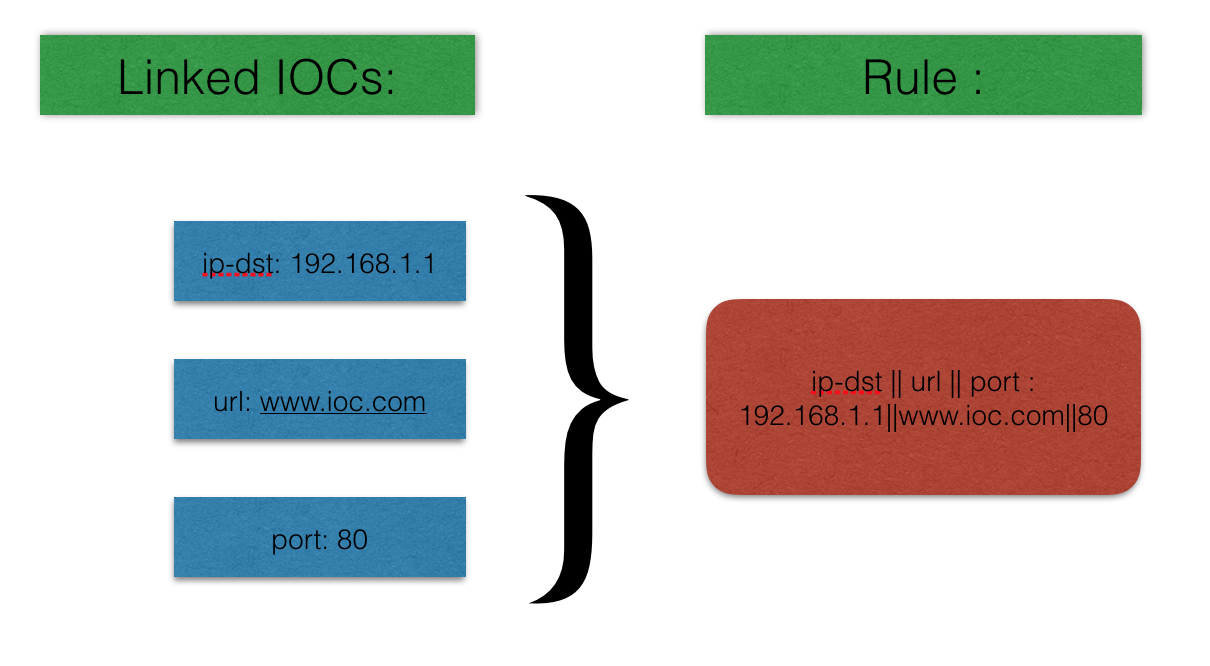
\includegraphics[scale=0.5]{res/ioc-rules}
	\caption{IOCs transformed into a rule}
	\label{IOC-To-Rule}
\end{center}
\end{figure}
\improvement{Not Combined IOCs But RELATED}

Rules as created can be directly checked on computers but they do not fit with our model yet as every values are still in clear. To solve this problem, they decided to hash the values concatenation while still keeping the structure (e.g. ip-dst||port) in clear.\\
The structure is what makes it still usable as it says the user which are the values they need to try against the rule.\\
The only additional computation is that the user needs to hash his values each time he tried to match the rule.\\
In this way, we are still really close to the hashstore previously explained but with the advantage of beeing able to individually store and share rules. We still lack some protections since every individual variable can only take a limited set and we still do not get back information while there is a match.\\
For solving that, they are using a non secret salt value chosen at random for \textbf{each} rules (IOC). Besides that, the attack time can be increased as well thanks to the cryptographic hash function used. The second part is really affecting the honest subscriber performance as well but is needed to slow down enough an attack for small data.\\

They didn't stop there, considering all these ideas, they have added the possibility to include a Course Of Action (COA) message with each rule. This is the real advantage compared to other techniques. The output is precise, there are neither false positive nor false negative and additionally, a match can give information to the honest user.\\ To do so, instead of hashing the combined values, they use it as input for a key derivation function (KDF) that generates a key used for encrypting a message.\\
Thus this new type of rule, instead of just obfuscating the data, contains the type of value (as before), the salt used for the rule and the encrypted message.\\


\begin{figure}[h!]
\begin{center}
	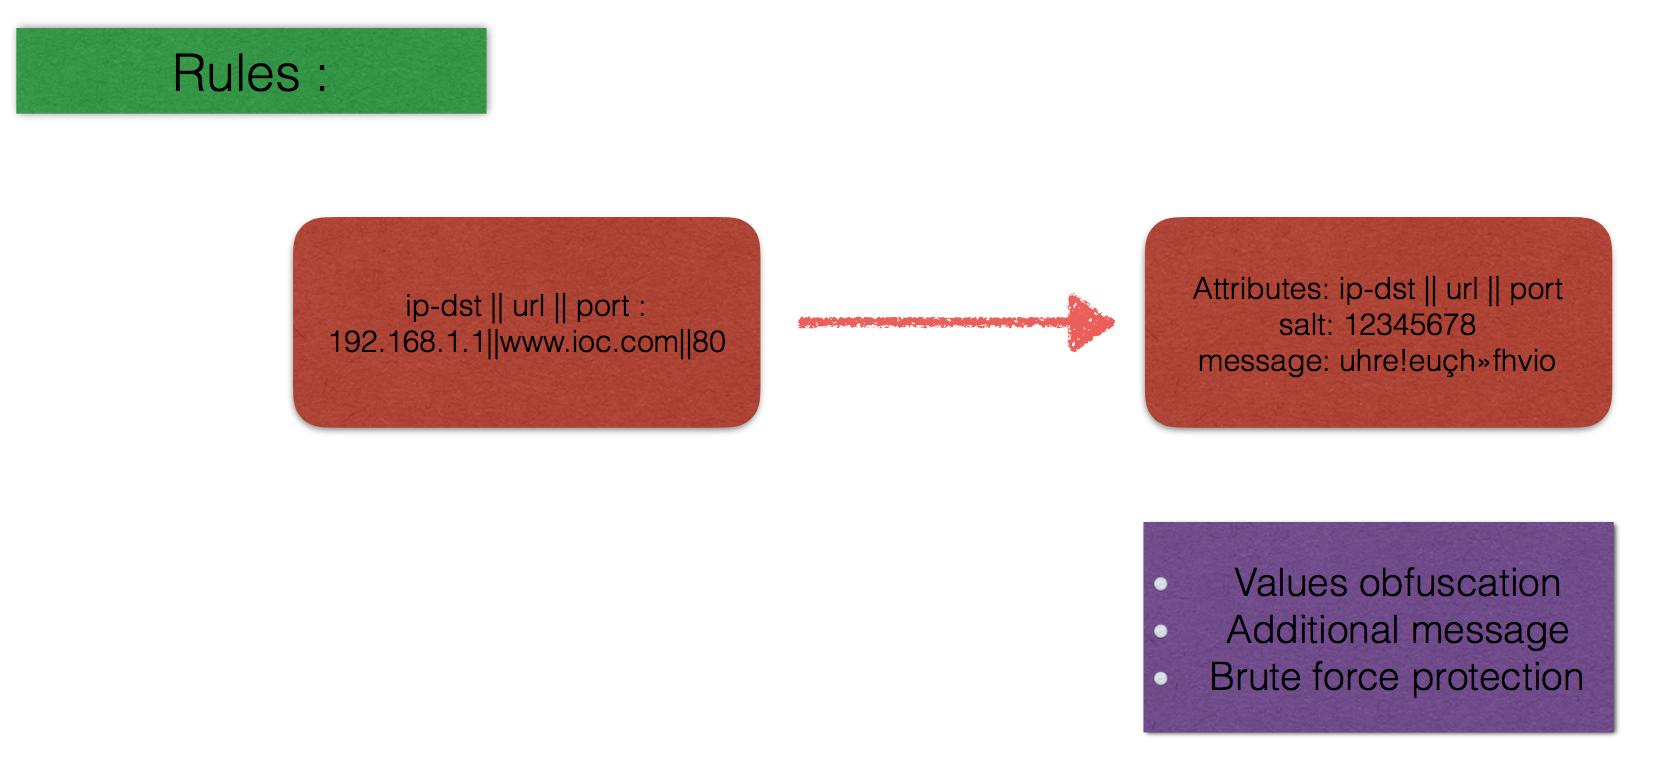
\includegraphics[scale=0.5]{res/obfuscation-rule}
	\caption{New format for the rules}
	\label{Obfuscation-Rule}
\end{center}
\end{figure}


This pseudo code shows how to generate a rule from the IOCs:

\begin{center}
\begin{boxedverbatim}
Function createRule(AttributeTypes, values, message, Token):
        pass = '||'.join(values)
        salt = GenSalt()
        key = kdf(token + salt + pass)
        message = 16 * '\x00' + message
        encr_message = encrypt(message, key)
        return dictionary(attributes=AttributeTypes, 
                            salt=salt,
                            ciphertext=encr_message)
\end{boxedverbatim}
\end{center}

Then, this pseudo code explain how to check values against one rule:
\begin{center}
\begin{boxedverbatim}
Function matchRule(dictianary(type -> value), rule, token):
        pass = '||'.join(values in rule.attributes)
        key = kdf(token + rule.salt + pass)
        if (decipher_16first_bytes(rule.message, key) = 16 * '\x00'):
                return decipher(rule.message, key)
        else
                return notMatched
\end{boxedverbatim}
\end{center}


Trust is one of the major problem in information sharing and is discussed in all standards, guides and articles. Here they have an attempt of solution that could really works. As a user cannot normally decrypt the complete rules data set, if for each generated rule, we add a source identifier in the KDF. This results in the ability to track the origin of a leak. \\
Even if it is a small add, I'm intimately convinced that it could help organizations to decide sharing more confidential data as they could turn themselves against the leakage source in case of problems which could limit the cost damage as well as the reputation damage. Moreover, in MISP there is also an identifier that could be used and which is called a Token.\\

In their implementation, they are using both HMAC and PBKDF2 for the key derivation function. I had the opportunity to exchange emails with the authors of the paper that prefers the HMAC algorithm as it is designed to give a pseudo random key in just a single iteration and that it has been deeply analyzed \cite{cryptoeprint}. While PBKDF2 is generating random keys that becomes more secure as the number of iterations increases. Moreover, the behavior has not been described (to the best of our knowledge) in academic paper even if there is a NIST recommendation on its usage.\\
They also used an AES encryption scheme.\\

Their proof of concept code is available on their repository, \url{https://github.com/CRIPTIM/private-IOC-sharing}. 


\section{My Implementation}
The article of Tim van de Kamp et al. gave me the starting point I needed as the code was available and under the MIT license. I've thus created two basic scripts starting from theirs where I've written it back to fit with MISP. At first, I've kept exactly the same scheme as they are.\\
The first step was to retrieve data from MISP, either from the web API, or by a direct connection towards the mysql database.\\
Then I've improved the code with different new functionalities and realized that, on the contrary of all university projects we had, the project needed to often be completely refactored to allow additional features and to keep it simple for an external user to understand how it works. I will thus go through theses different implementation parts in the next few sections.\\

\subsection{Get data from MISP}
To create the rules with the encrypted messages, we first need to get a subset of IOCs contained in MISP that are destined to IDS. \\
For doing so, there is tree possibilities, the first one is working with the MISP webAPI while the second one is directly connected to the mysql database. \\
A third that directly reads from a csv file had been added to be able to select what should be shared and for a testing purpose.\\
The recommended mode will be with the web API, but as rules will be generated directly on the server, it could be more efficient to use directly the MySQL connection.\\

For making automation request on MISP, they have implemented a python library called PyMISP. The first idea was to use it but it was finally not interesting to import the whole library only to make one request. That is why, I've changed the system by making myself the request to the automation API by using the requests python library and the MISP token referenced in the configuration file.\\

The virtual machine has been a great utility to understand how it is working, and especially how the database is structured. I've also added additional check like verifying that the email address specified is the one related to the token when the MySQL connection is used.

\subsection{Parsing logs}
The idea was to test the system with log files as I did with the hashstore. First I tried to reuse the parser I've created but I tried to go to deep in the analyze and it has bad performances as well as a lot of particular cases that were not working.\\
I thus changed my mind and used logstash and redis to store the parsed log. \\
It also has the big advantage to be modular and only a new configuration file is needed to parse any other type of log files.\\
Besides that, I'm storing the data inside a redis queue and polling on it in the script for trying to match a rule. \\
\improvement{ Add details, schemas, Structure explanation, ...;}

\subsection{Multiprocessing}
When there are a lot of logs, doing one by one take too much time, but we can test simultaneously more than one log line at the same time by creating processes.\\
Also it is important to point out that I've started this by trying to use threads but, as I'm using the cpython interpreter, it is impossible to have two program running simultaneously due to the Global Interpreter Lock (GIL). That is why, I finally chose to create a pool of processes instead.

\improvement{Data could be shared on redis instead}
\subsection{I/O and Rule Size Optimization}
In the implementation of Tim van de Kamp et al., for each rule, they created a file to store the rule. \\
I can understand it in the point of vue of a proof of concept but it is a real bad idea as in UNIX systems, each file has a minimum size of 4k. Already with 6300 events each one possessing 153 attributes in average, it is easy to see the problem coming. Moreover, the I/O were really slowing down the system. \\
These problems were easy to solve. Create a complete csv file for all rules. But is still not a solution because it would mean that we should load everything in memory even if we don't use everything. That is why I finally chosen to have one csv file per type of IOCs.
\improvement{Plus de détails}
\subsection{CSV or TSV?}
This is a really small modification but makes files more readable and avoid existing coma in the data to make the parsing not working.

\subsection{On URL Normalization}
The goal of the system is looking for matches in MISP data. But off course, if an event has for Uniform Resource Locator (URL) www.ioc.com I would like http://www.ioc.com, http://www.ioc.com/, http://www.ioc.com:80/, ... To match as well.\\
I first dug a little into URL normalization like the standards and techniques already used in practice. I've realized that normalization is difficult as, in the standards, they want URL to always work after, and really be the same. For example http://www.ioc.com is not https://www.ioc.com while in matching, I absolutely don't care and I would like to both trigger an alert.\\
Besides that, there are standards on URL normalization [RFC 3986] that contains either normalizations that preserve or usually preserve the semantic of the URL but none that does not preserve it.\\
Standards are thus focus on keeping the number of false positive near to 0 but it has for impact to miss a lot of real positive and we cannot afford that.\\
I've thus found this paper \cite{lee2005url} which was focus on url normalization and that goes beyond standards normalization steps like case sensitivity in the path, the last slash symbol at the end of the path and the designation of the default page (index.html, ...).\\
Besides that, a great summary of all these standardizations steps is available on wikipedia \cite{wikiNormalizationURL}.\\
In the implementation, I've used the python library url\_normalize:
\begin{itemize}
\item[•] Take care of IDN domains.
\item[•] Always provide the URI scheme in lowercase characters.
\item[•] Always provide the host, if any, in lowercase characters.
\item[•] Only perform percent-encoding where it is essential.
\item[•] Always use uppercase A-through-F characters when percent-encoding.
\item[•] Prevent dot-segments appearing in non-relative URI paths.
\item[•] For schemes that define a default authority, use an empty authority if the default is desired.
\item[•] For schemes that define an empty path to be equivalent to a path of "/", use "/".
\item[•] For schemes that define a port, use an empty port if the default is desired
\item[•] All portions of the URI must be utf-8 encoded NFC from Unicode strings
\end{itemize}

I thus added some additional steps like:
\begin{itemize}
\item Removing directory index : {default.asp, index.html, index.php, index.shtml, index.jsp, default.asp}.
\item Remove the fragment (\#...) which is never seen by the server.
\item Removing the protocol {http://, https://}.
\item Removing  “www” as the first domain label.
\item Removing the "?" when the query is empty.
\end{itemize}

\subsection{Only PBKDF2}
While I was adding stuffs, it becomes more and more difficult to allow all these possible choices, I've thus started by limiting the key derivation function (KDF) choice to PBKDF2 which is not the author advised one but allow to parametrize the difficulty for an attacker to brute force some small data.\\
But in the opposite we cannot have a small number iteration if we want the key to look random. Which is finally the intended use as we want to slow down bruteforce attacks.

\subsection{library: Pycrypto towards Cryptography}
While discussing with Tim van de Kamp by email, he said that if he had to start over, he would choose the cryptography library \footnote{https://cryptography.io/en/latest/} instead of pycrypto because it seems to be a more professional implementation.\\
I thus have made some research on it. There are some discussion about it but \url{libhunt.com} gives this table \ref{cryptoLibraries} where we can see that even if pycrypto seems better written, the cryptography library is more up to date and still with a lot of activities.\\
Besides that, I found the library well defined and really easy to use that is why, I've chosen to refactor the code with this particular library instead.


\begin{table}[h!]
\centering
\caption{Cryptography Libraries Comparison}
\label{cryptoLibraries}
\begin{tabular}{|l|c|c|}
\hline
                                                                  & \multicolumn{1}{l|}{{ \textbf{PyCrypto}}} & \multicolumn{1}{l|}{{ \textbf{Cryptography}}}                                              \\ \hline
Popularity                                                        & 7.2                                          & \textbf{7.3}                                                                                  \\ \hline
Activity                                                          & 0.0                                          & \textbf{9.0}                                                                                  \\ \hline
Stars                                                             & 1 345                                        & \textbf{1 431}                                                                                \\ \hline
Watchers                                                          & \textbf{103}                                 & 86                                                                                            \\ \hline
Last Commit                                                       & about 3 years ago                            & \textbf{\begin{tabular}[c]{@{}c@{}}7 hours before checking\\ on the 13 April 17\end{tabular}} \\ \hline
\begin{tabular}[c]{@{}l@{}}Code Quality\\ (L1 to L5)\end{tabular} & \textbf{L4}                                  & L2                                                                                            \\ \hline
\end{tabular}
\end{table}


\subsection{Structure Improvement}
The code was becoming less and less clear to understand and as I wanted it to be modular for the cryptographic system used. I've decided to completely re factor the code.\\
The used structure is as following:
\begin{itemize}
\item src: Source code.
\item conf: Configuration files.
\item res: All downloaded useful resources like the csv downloaded from MISP.
\item rules: Rules generated.
\end{itemize}

Inside src, there is also a crypto subdirectory in which are located all cryptographic functions in the different possible schemes implemented.

\subsection{Top Configuration File}
Instead of having a lot of configuration files as when I started, I've gathered them back in one general file where we only have to fill what will be used (Specified in function).\\
The configuration file is divided in categories and is read thanks to the configparser python library.

\section{Chosen Cryptographic System}
The idea of the generalization was to add module for handling the way data are stored / encrypted, we can use completely different cryptographic systems later called schemes. In this section, I will discuss my implementation choices for each schemes implemented.

\subsection{PBKDF2}
This is the basic system for which all the structure had been optimized and had been thought for. In this section, I will thus briefly introduce these two sequence diagrams to help the understanding the system:
\begin{figure}[h!]
\begin{center}
   \begin{minipage}[c]{.46\linewidth}
      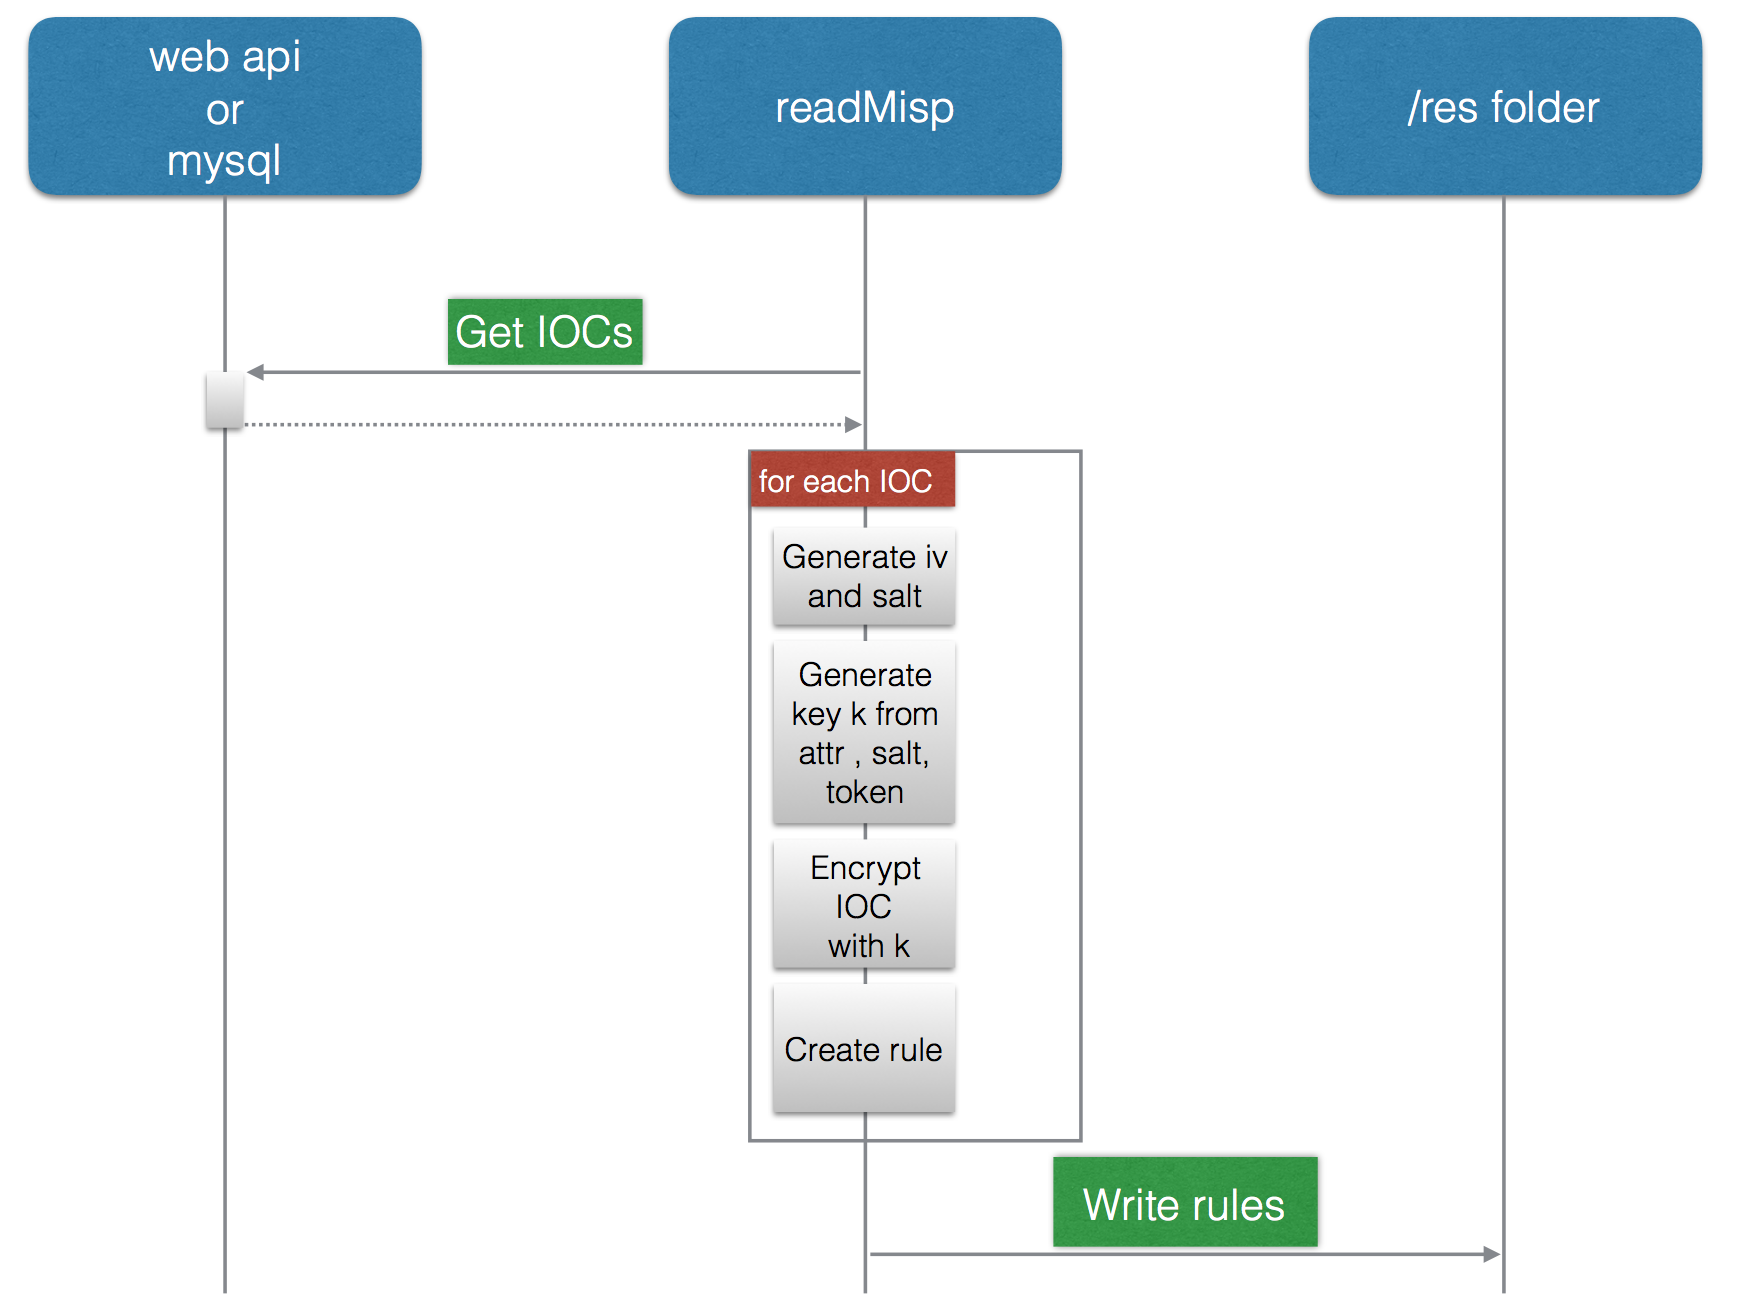
\includegraphics[scale=0.25]{res/seqDiagramRead}
   \end{minipage} \hfill
   \begin{minipage}[c]{.46\linewidth}
      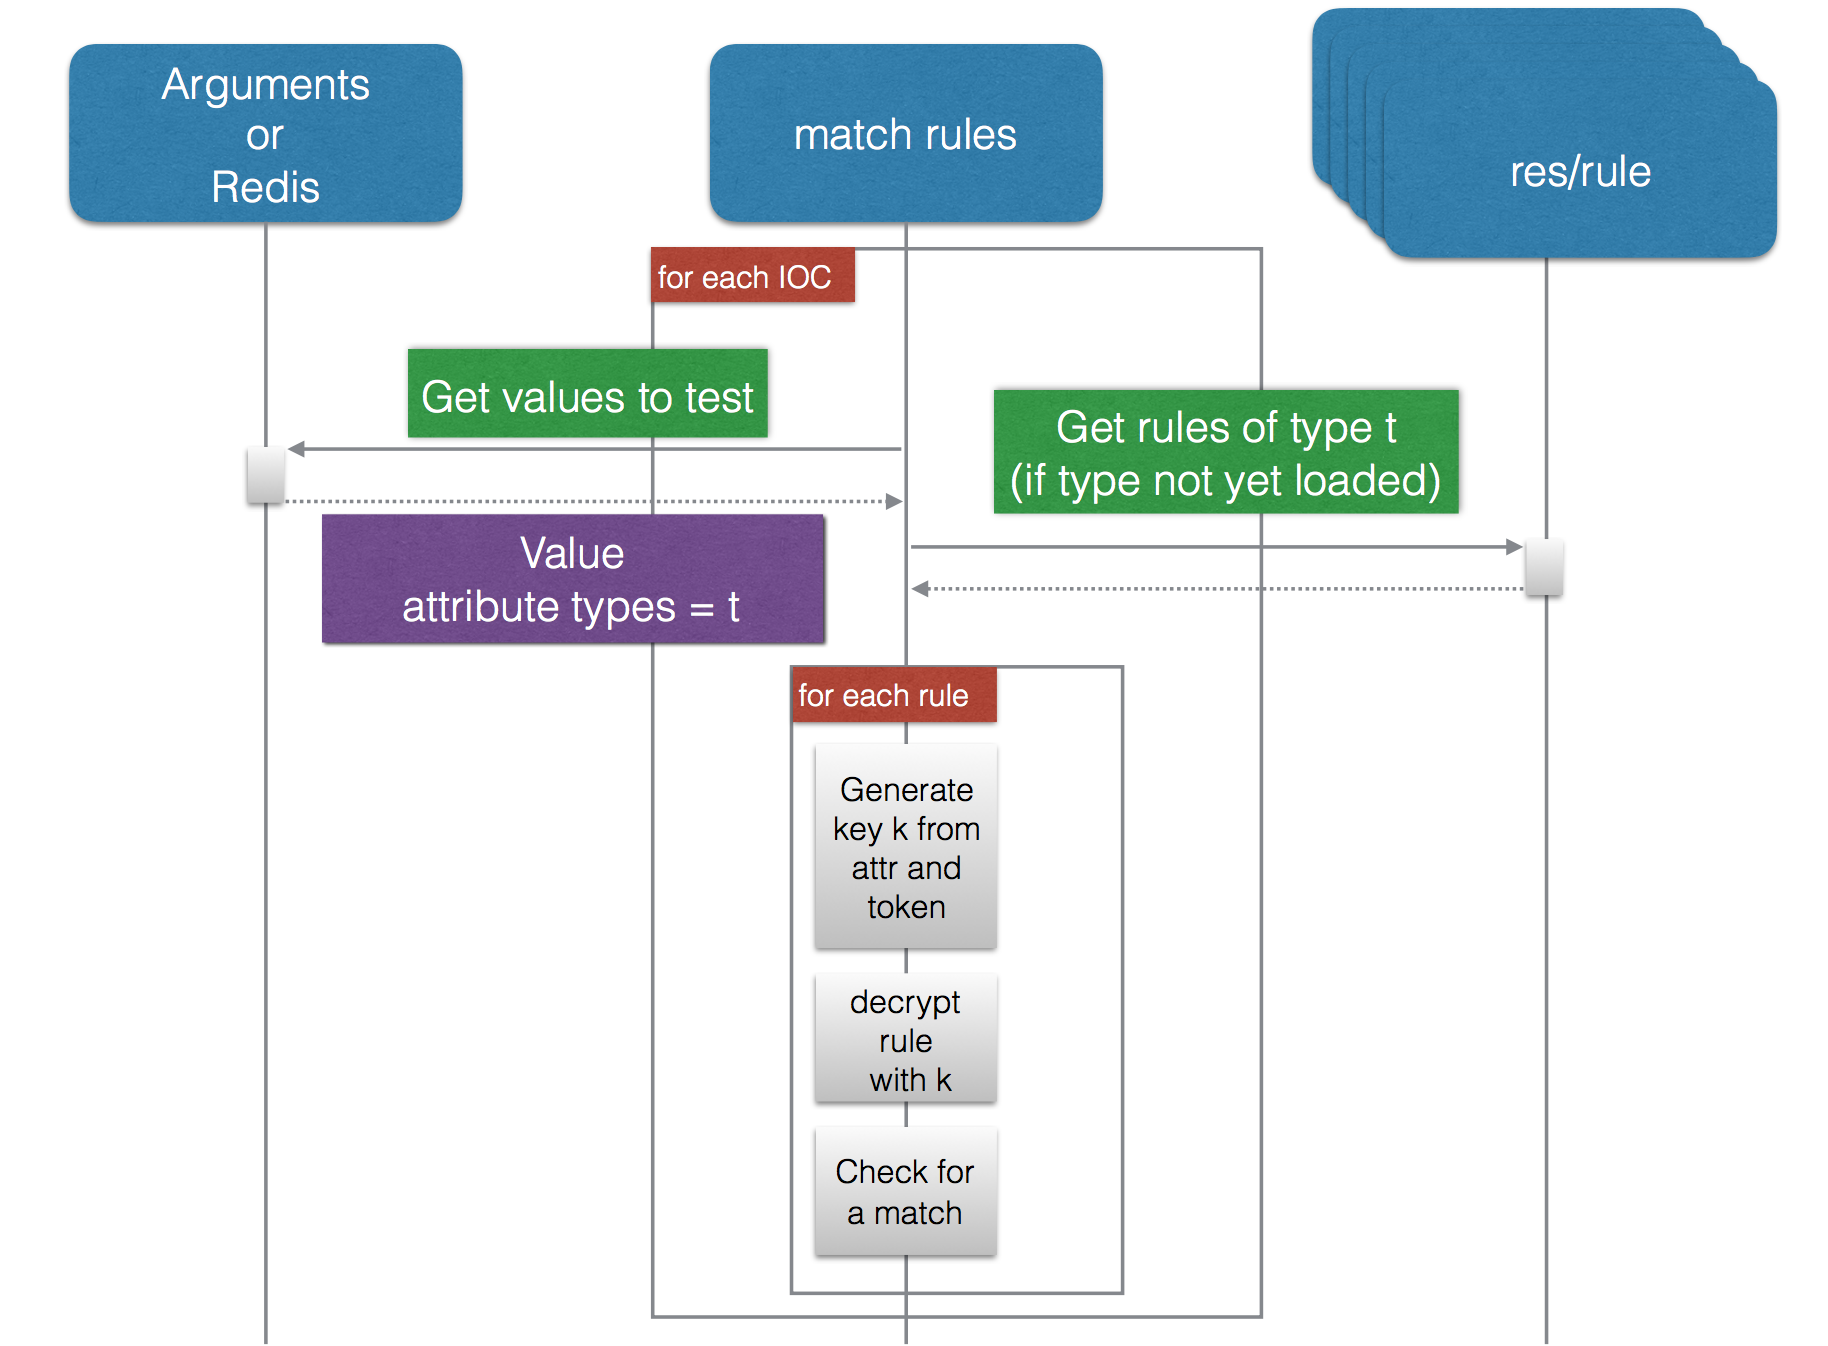
\includegraphics[scale=0.25]{res/seqDiagramMatch}
   \end{minipage}
\end{center}
\end{figure}

For the cryptographic system, there is also an small difference in the rules that allow a really faster matching.\\
Instead of directly encrypt the whole message, I've decided to divide it in two parts (easy to do with the cryptography library). The first is the ciphertext-check and the other one is the ciphertext. The ciphertext-check is simply the first bock of the encrypted message. It is used only for matching, decrypt it must result in only zeros if there is a match.\\

For this algorithm, the user must choose an important meta parameter that will determine the "security level". This meta parameter is the number of iterations for the key derivation functions.\\
In 2000, the RFC advised 1000 iterations for password storing. In 2015, OWASP password storage cheat sheet \cite{van2015password} advised about 10 000 iterations while NIST recommends on its appendix A.2.2 of its guide \cite{turan2010nist} to use as many iterations as it is possible with the needed performances.\\

Some additional analyses can be make on the ability to sustain an attack, the article make by the CryptoSense\footnote{\url{https://cryptosense.com/parameter-choice-for-pbkdf2/}} website is really well documented.\\
They have analyzed previous work and have done some estimation for 2015. Their approximation is more a guess than anything else and I wouldn't dare trying their approximation for 2017 but I will nevertheless show their results to get a rough ideas of what could be the time to crack a password from a key generated with PBKDF2 (AES + SHA-1):\\
\begin{table}[h!]
\centering
\caption{My caption}
\label{my-label}
\begin{tabular}{|c|c|c|c|}
\hline
Password Complexity & Estimated Entropy (bits) & 1 000 Iterations & 10 000 iterations \\ \hline
Comprehensive8 & 33 & 4h46 & 47h \\ \hline
8 random lowercase letters & 37 & 12h & 5 days \\ \hline
8 random letters & 45 & 123 days & 3 years 5 months \\ \hline
\begin{tabular}[c]{@{}c@{}}8 letters + numbers + punctuation \\ OR \\ 4 random Diceware words\end{tabular} & 52 & 325 years & 3250 years \\ \hline
\end{tabular}
\end{table}

\subsection{Bcrypt}
The implementation with Bcrypt is similar as my implementation with PBKDF2. It is a password hash function based on the Blowfish cipher. It also incorporates salts to be protected against rainbow table attacks (TMTO).\\
It has also advantages as being more configurable and is more efficient against GPU attacks. It also seems better to use but the NIST recommendations are still about PBKDF2.\\

On the other hand, the time complexity of the implementation is not the same as for PBKDF2.\\
The problem with this algorithm is that they only consider the 72 firsts characters of the password for the key generation. It can seems a lot but even this url \url{https://translate.google.com/#fr/en/72\%20caract\%C3\%A8re\%2C\%20ce\%20n'est\%20pas\%20beaucoup} is 88 characters long. This means that if we add the token at the end (like in PKKDF2) it will not be included. On the other side, if we first put the token before the data, an attacker would know that the 40 firsts characters will always be the same and moreover, there are only 32 characters left for the data which is not enough even for an IPv6.\\
As the goal was that the whole string has an impact to the key generated as well as the token to have an impact on all bits. The solution was thus obviously to hash the concatenation of the value with the token and then seed this fingerprint to the key generation function.\\

We also know that such key derivation function are aimed to have a time complexity that growth exponentially with the number of characters. Here every element can be considered as a 72 characters element (has the hash is longer) which means that with this technique, it can take really longer to check IPs in the system and so for bruteforcing as well. It thus need to be taken into consideration before choosing the number of iterations for small data.


\subsection{Bloom filter}
In this section, I will argue the choice for python-bloom library. This choice was actually a way more complicated than it could be as, I think it is not the fastest implementation.\\
But first, to understand my choice, we need to know what I really was searching for. I needed to find a way for avoiding brute forcing the database, but, on the other hand, I want it to be really fast for a common user. Thus Bloom filters already take car of the first part so, I only needed to find a fast implementation.\\
I also wanted the system to be storable in files without any additional information.\\
So the first I've found was to use bloomd server with a python client. But, it would means that we would have to install all these things which seems not really interesting. But why not using redis to store data ? It is fast and there was a really fast implementation of bloom filters in python for redis (actually in c interfaced with python) call pyrebloom. But the code was really complicated and not easy to read. Moreover, I discovered that they are keeping additional information on keys to be able to remove elements. that, without forgetting the fact that it doesn't seemed savable in a file make me drop this implementation.\\
I've finally found the python-bloom library, It seems less efficient but well implemented, without any additional state and a way to save the bloom filter.\\

For the bloom filter, I've got different ideas, first, I need to implement the bloom filter as a tsv file. But, I also need it to be loaded each time. For this, I've added a special joker rule that is always loaded if it exists.\\
On this first implementation, I would like to have only one bloom filter for the whole data set. I could have implemented a bloom filter for attributes but as it is fast enough, it would use less memory and will be more efficient to use only one bloom filter.\\



\subsection{Bloom filter used as to improve performance of Key Derivation Functions}
Key derivation function are working to slow down a brute force attack. This is working really well as the complexity of a brute force attack time complexity increases exponentially with then length of the string to "crack". On the other hand, if we know exactly the data we are looking for and that there is a small set of different values. We cannot do anything against it. \\

So if we came back on a longer sized data like URLs, brute forcing them (if we are not looking especially for a value) is close to impossible and making the task easier for a user makes the task easier as well for the attacker. But it can still be nearly infeasible for an attacker to brute force the whole dataset while making the system a way more faster for the user.\\

With this idea in mind, I've used both type of implementations to create key derivation function improved with a bloom filter. The bloom filter avoid decrypting each rules if no rules contains the data we are looking for. \\
And, on the other side, when there is a match, rules can be used to get back the information needed to retrieve the event information from MISP. \improvement{Add an explanation on the message generated and how we could use it to find information on an event}\\

This is a serious advantage for matching. In function of the bloom filter false positive rate the system could me made a lot faster. So much faster that we could use it directly as an IDS that could updated time to time and that could work on computers, logs and that could work stand alone to generate reports on event that could affect a system.\\
The previous system was first aimed to be used like that but we a recommended number of iterations, the system was too slow to use in that way as data to check accumulates at a much bigger rate than the system need to look through all rules.\\

Thus increasing the speed can be done by decreasing the rate of false positive of the bloom filter but what if an attacker is only interesting in knowing the element belonging to the data set ?\\
The bloom filter could give him all the information he needs. This is the reason why we can not take a too small rate for the bloom filter.\\


\section{An other KDF}
An open competition called Password Hashing Competition (PHC) started on 2013 to meet the needs of a standard password hashing algorithm.\\ 
It ended in 2015 by selecting the winner as Argon2 and also a special recognition to some other algorithms like Catena, Lyra2, yescrypt and Makwa.\\
Argon2 was designed in the University of Luxembourg and there is three versions:
\begin{itemize}
\item[$\bullet$] Argon2d maximizes resistance to GPU cracking attacks.
\item[$\bullet$] Argon2i is optimized to resist side-channel attacks.
\item[$\bullet$] Argon2id is a hybrid version out of Argon2d and Argon2i.
\end{itemize}

There are two available libraries that implements Argon2 which are passlib and argon2\_cffi.\\
This could be interesting to use it instead of bcrypt or pbkdf2 but unfortunately, the two existing libraries have directly integrated the salt generation. \\
The only way of using it for now would have been to take a salt of length zero and to generate the salt by myself. \\
But I'm not sure that it would keep it's security value doing so.

\chapter{Results}
Finally, the most interesting part is coming, is it really working? Is the additional computation worth it? Can we trust this system with our data ? Could with improve the code for the computation time ?\\
This final chapter will try to answer those questions. With the code restructuring, I think I have succeeded in creating code easy to understand but there are still some tricky hacks that I will need to get rid of for make easier addons creation.
This first part will be on understanding the used dataset, then I will focus on the code profiling to understand which parts could be improved.\\
Then I will explain a set of benchmark to try to show the interest of this system.\\
Discussion on the security of the techniques and their usability will serve as a nice conclusion.\\

\section{Dataset}
The objective was to make all data available if additional computation must be done or this work must be continued. For that, following the same reflection as with the starting screen-shots, the data directly inside the virtual machine are TLP white and are available for every one as we can directly download them on the CIRCL website : \url{https://circl.lu/services/misp-training-materials/}.\\
Thus I've used these data instead of the one directly from an instance. Even if there are a lot less data here, the computations and analyze give the necessary idea.

\section{Code Profiling}
This section is divided in three parts, a deeper understanding of the code work flow is needed to understand where the time is lost during the execution. Then, the code will be profiled for two different executions, the first is aimed to compare the time of the key generation with only one iteration. That give a right comparison point between the different functions and the second will be with 1000 iterations to see how it occupies the time. 


\subsection{Code Flow}
As previously explained, a deeper understanding of the different work flow of the code are important to understand the later profile.\\
This explanation will be separated into the read, match and crypto part as crypto is used by both.

\subsubsection{ReadMisp}
\begin{figure}[h!]
\begin{center}
	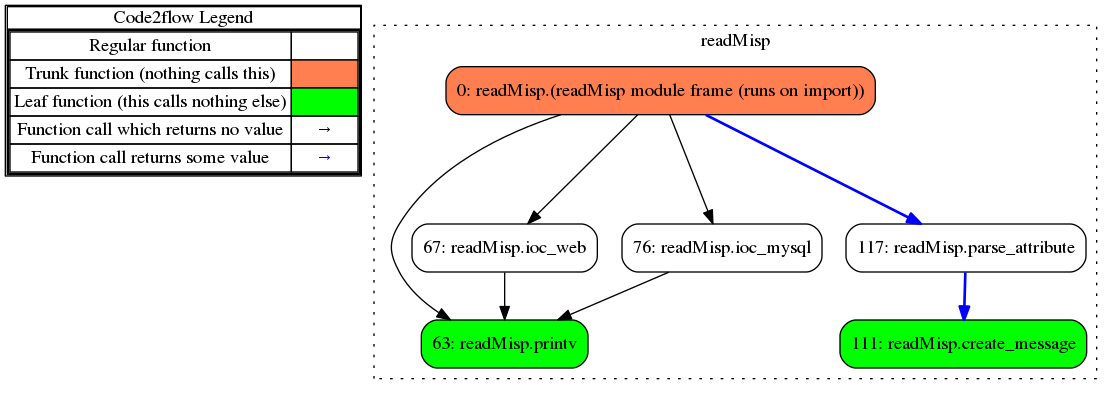
\includegraphics[scale=0.3]{res/flowReadMisp}
	\caption{Code2flow: ReadMisp WorkFlow}
	\label{code2flow-readMisp}
\end{center}
\end{figure}
ReadMisp (fig. \ref{code2flow-readMisp}) will first retrieve the data, either via the web API or the MySQL connection. The advantage of the MySQL is the speed for two reasons, first, there are no data transformation as we request the data as it is stored and secondly, in general, the MySQL server is accessible only from the server which means that there is less network delay.\\
On the flow chart, we can also see the function printv which is a call to print only if the program runs in verbose mode.\\
Once the IOCs available, the attributes are parsed and the message is created.\\
For the parsing is the real creation of the rule, which is done in several steps:

\begin{itemize}
\item[$\bullet$] Values from Misp are split and associated with their type in a dictionary.
\item[$\bullet$] URL are normalized.
\item[$\bullet$] The message is created.
\item[$\bullet$] The Crypto package is called to create the rule.
\end{itemize}

In order to be modular, all the code for rule creation is separated. Each time that the program is started, it goes to the configuration file to see which Crypto module to load from the crypto package.\\
All modules need to implement the interface (interface.py) and then must be add in the choose\_crypto.py.\\
For an example, the work flow for the PKKDF module is available on figure \ref{code2flow-pbkdf2}.

\subsubsection{MatchRules}
\begin{figure}[h!]
\begin{center}
	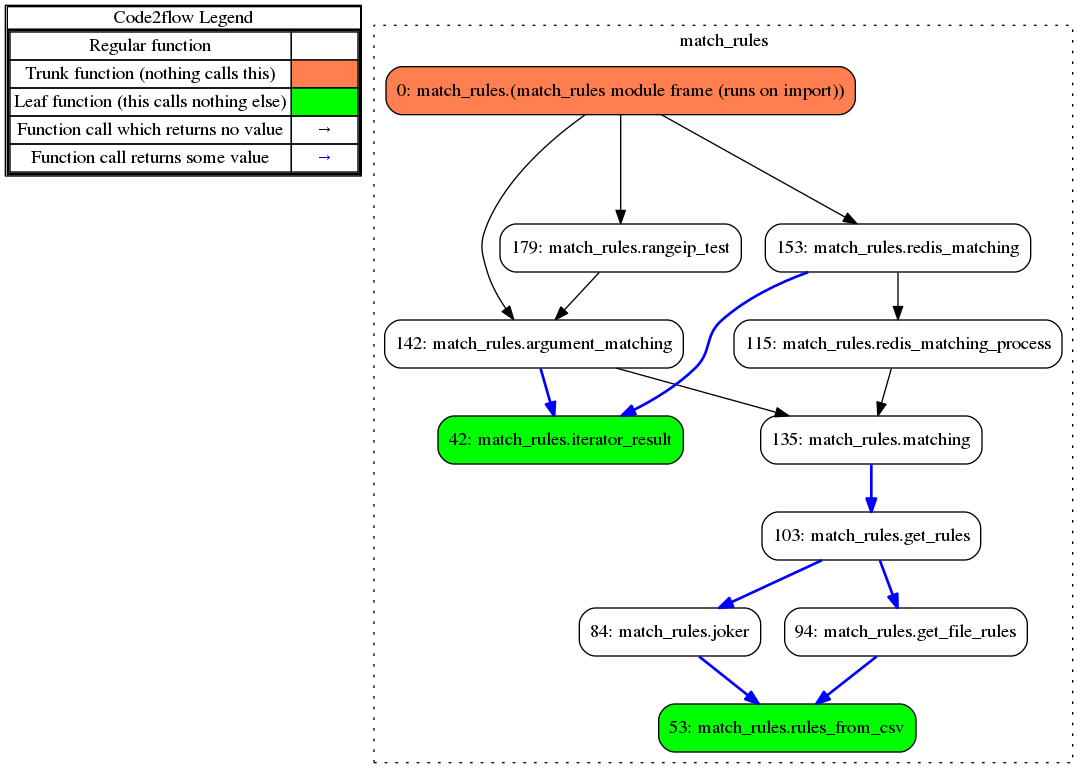
\includegraphics[scale=0.3]{res/flowMatchRules}
	\caption{Code2flow: MatchRules WorkFlow}
	\label{code2flow-matchRules}
\end{center}
\end{figure}

Match rules has two really different ways of working, try to match an element from the arguments (argument matching) or from redis if the pipeline system with logs is used.\\
The additional rangeip test is just for testing purpose and will be further explained in the benchmark sections.\\

For redis matching, the only difference is that a pool of process running a redis matching process is used.\\
Each process is actually polling the redis queue for new logs and is then feeding them to the matching system.\\
In the other system, the arguments are directly seeded to the matching system.\\

The matching system is working in different steps, first, in function of the argument types, it will load and cache the needed rules.\\
There are two types of rules, the standards one are divided into files but, as I've added systems like bloom filter, it was easier to have a special file always loaded that I called Joker.\\

Once the rules loaded, for each attributes to check, the crypto module will try to decrypt each rules up to find or not a match.

\subsubsection{Crypto Module PBKDF2}

\begin{figure}[h!]
\begin{center}
	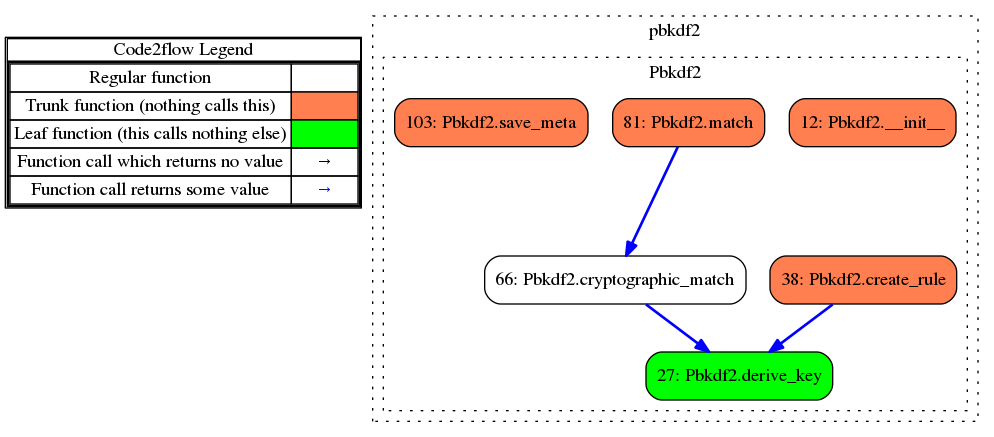
\includegraphics[scale=0.3]{res/flowPBKDF2}
	\caption{Code2flow: PBKDF2 Crypto Module WorkFlow}
	\label{code2flow-pbkdf2}
\end{center}
\end{figure}

\begin{figure}[h!]
\begin{center}
	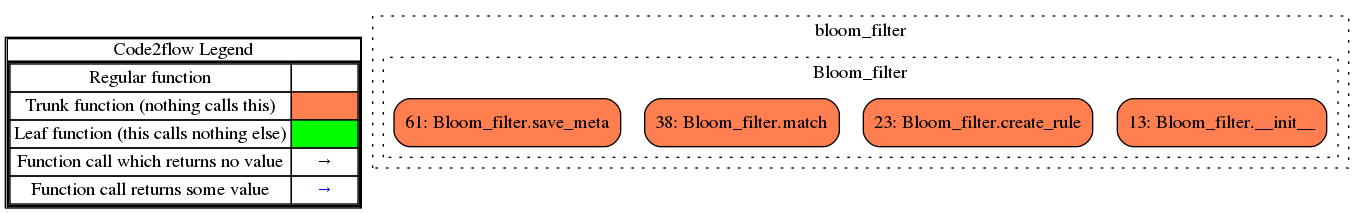
\includegraphics[scale=0.3]{res/flowBloomFilter}
	\caption{Code2flow: Bloom Filter Crypto Module WorkFlow}
	\label{code2flow-bloom}
\end{center}
\end{figure}

The crypto modules are responsible for creating and matching rules. In the particular case of the PBKDF2 module, it generate the keys and encrypt the message or try to decipher it.\\
I've additionally add the bloom filter chart as well to see the difference is small as they inherit the same interface.\\

As the types of file can differ from modules to modules, this is also the crypto module wich is responsible to save data and meta data files.\\
This part can take a lot of time as for saving the elements (as well as getting them) because we cannot afford problems inside the files like special characters to appear. So for that the idea is to use base64 encoding for the encrypted message, the salt (or nounce) and also the cipher-check argument (used for faster match checking).\\


\subsection{Profile of ReadMisp for 1 iteration}
We thus need to verify that generating the keys and encrypting/decrypting data is much more time consuming than everything else even with one iteration.\\
We should also do especially close attention to the normalization of URLs. Normalizations could be inefficient as I don't know how the library is implemented and moreover, I'm additionally iterating for searching regex after that.\\

For profiling the code, I've had some difficulties, first, I tried to use the vprof profiler as it seems to be the best and it was said that it supports python3.\\
But there were a lot of errors and I first didn't succeed in using it. I've thus tried to use a line\_profiler (only working with python2) then profiling which was really complicated to used. \\
I finally managed to use vprof with a little modification (to force it using python3) and I was really impressed by this tool that analyze everything. We can have graphs of the function utilizations, a line by line profiler but also a memory analyzer which can be really useful.\\

\begin{figure}[h!]
\begin{center}
	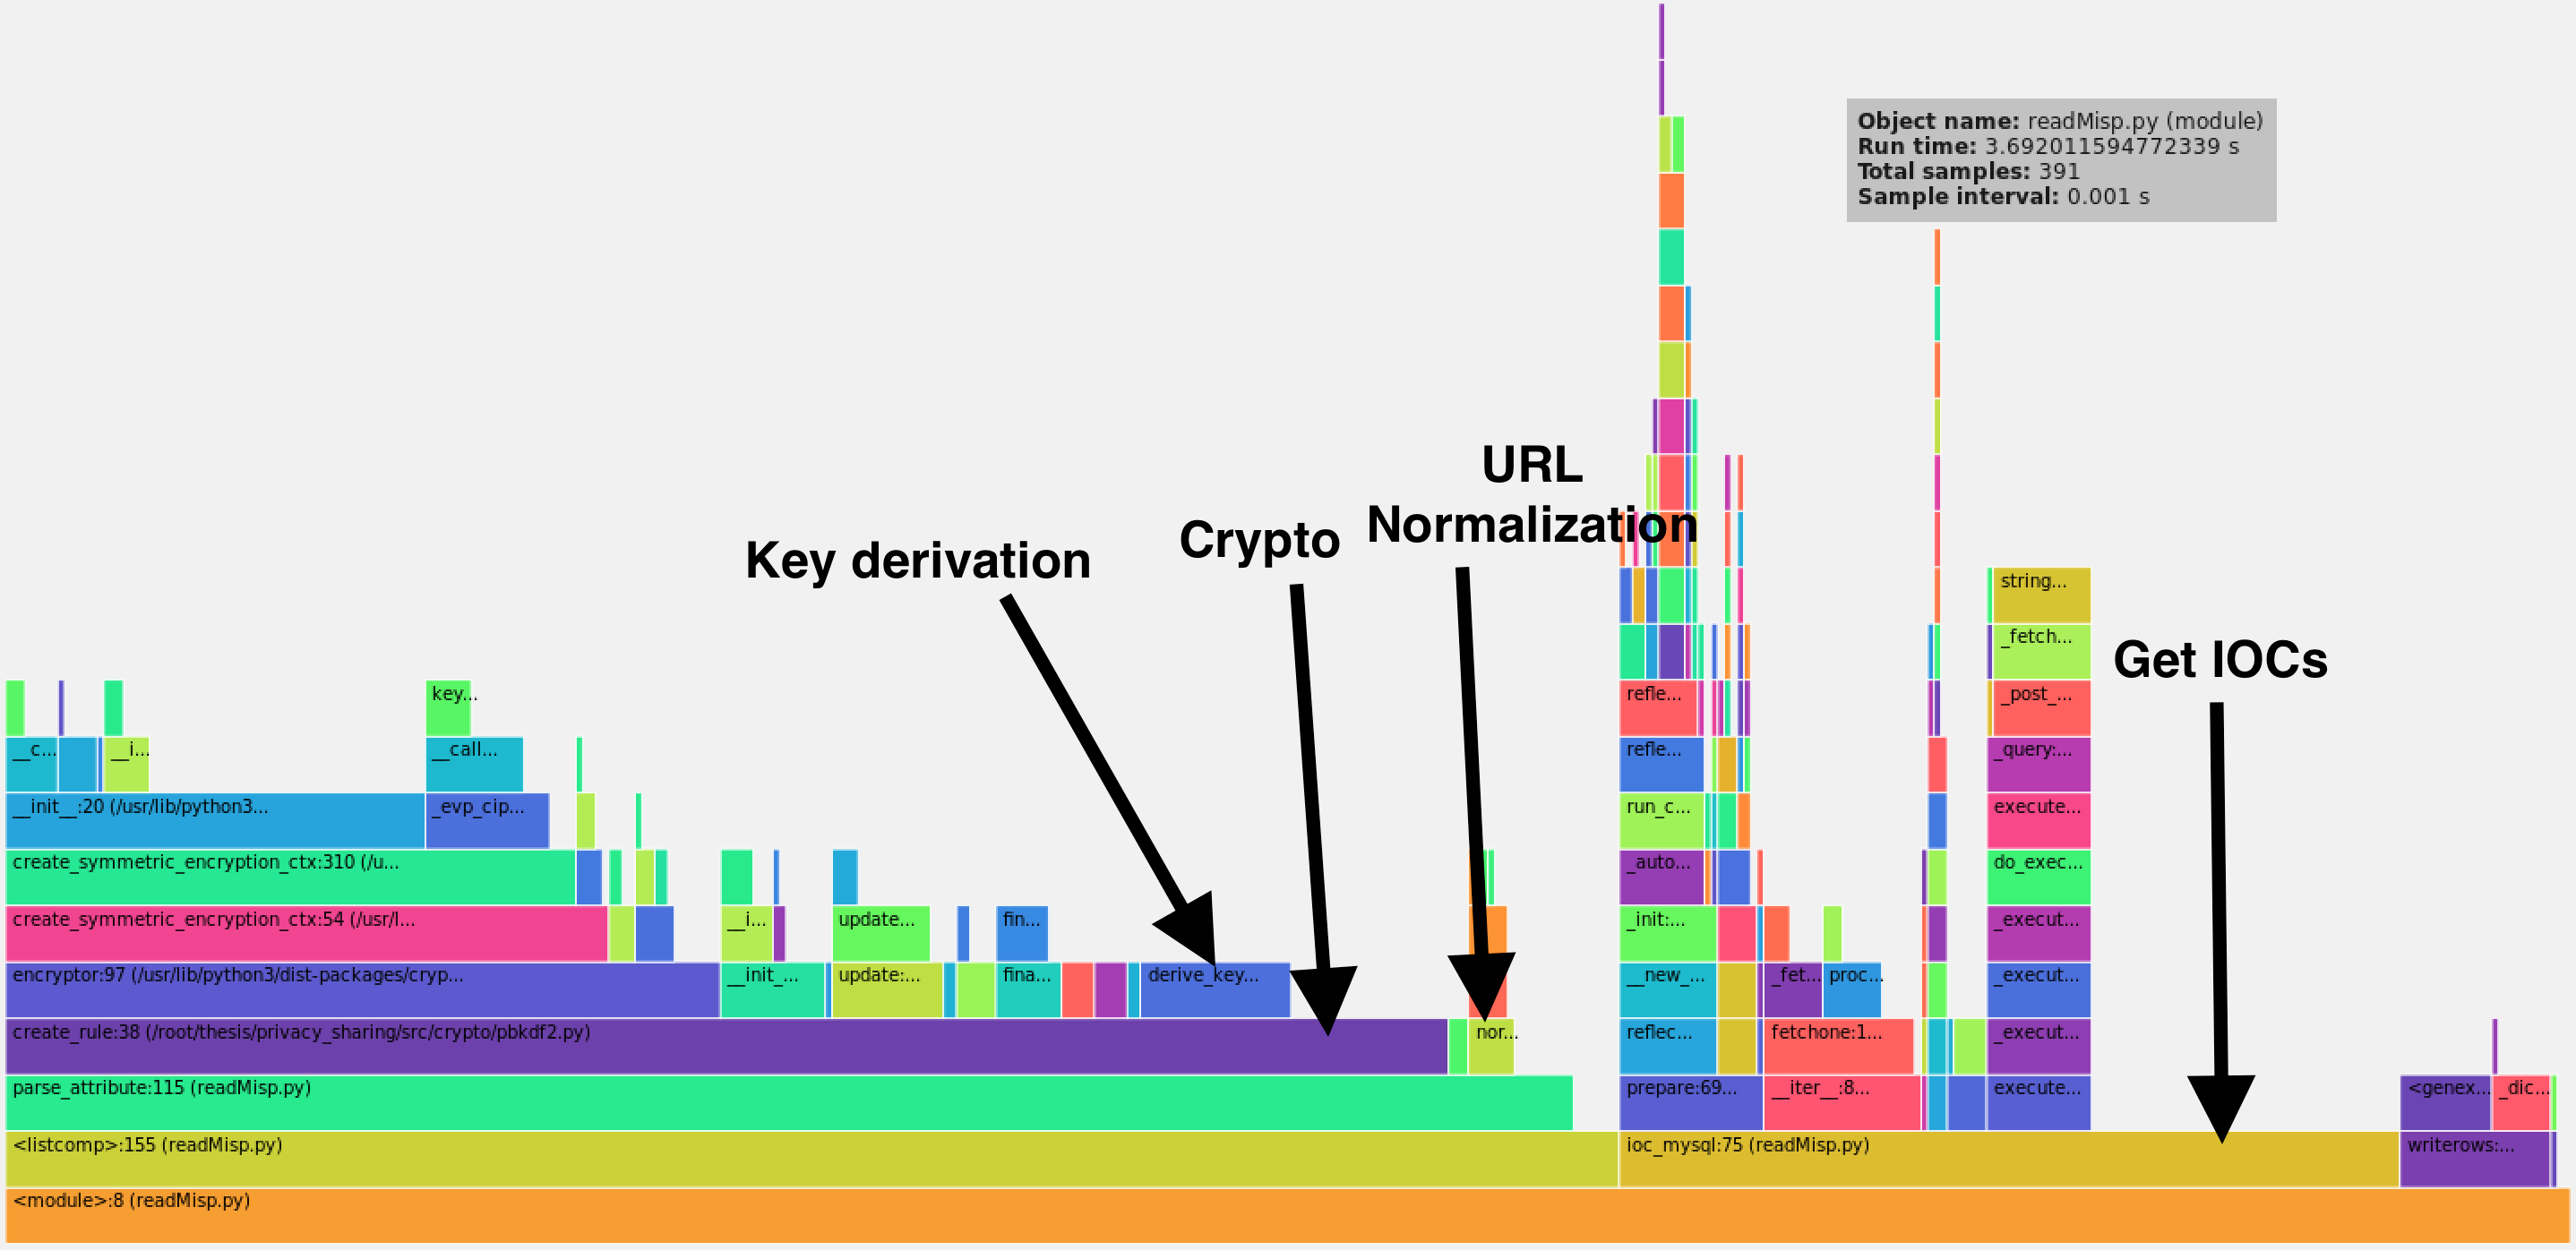
\includegraphics[scale=0.3]{res/profile-1iter}
	\caption{Vprof - Flame Chart Profile of readMisp PBKDF2(1 iteration)}
	\label{profile-readMisp}
\end{center}
\end{figure}

This graph \ref{profile-readMisp} shows that getting the IOCs from MySQL takes approximately one third of the time. And there, we also see that two thirds of this section are used directly for Mysql but the one third left is used for ordering and small modification of the format of some values. This could be slightly improved but this would not increase the average performance as we can see with 1000 iterations.\\
Then writing data to files (Rightmost dark blue) takes time but cannot be improved significantly.\\  
The first question about the normalization time is answered and we see that it shows that normalizations of URLs is already a small amount of time compared to one iteration for the key derivation.\\
We also see that in this particular case, the major part of the time is taken by the encryption of the messages.

\begin{figure}[h!]
\begin{center}
	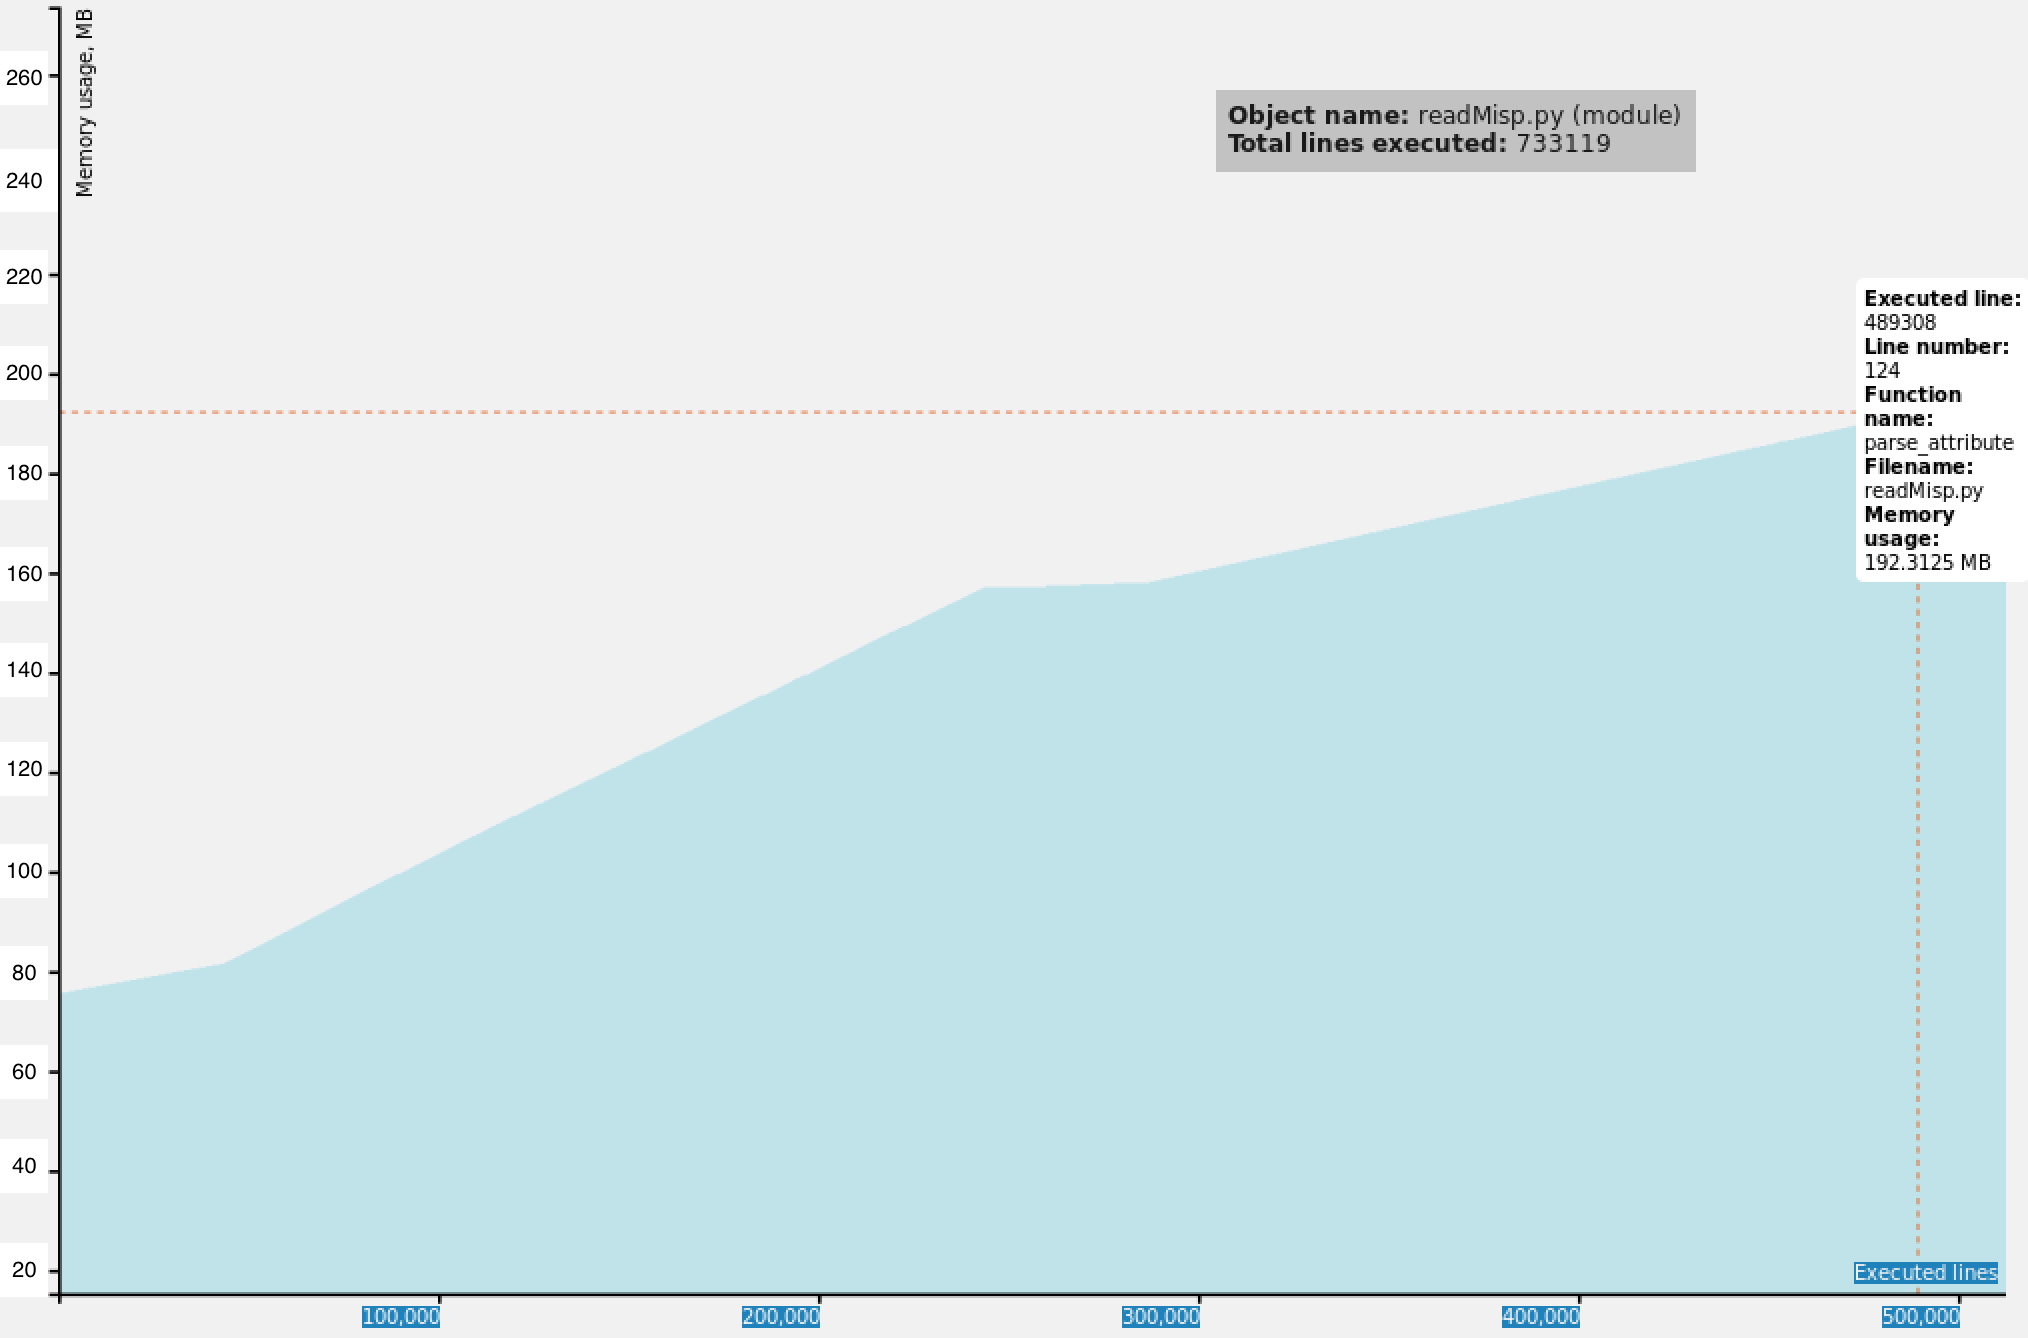
\includegraphics[scale=0.3]{res/profile-mem-readMisp-1iter}
	\caption{Vprof - Memory Chart Profile of readMisp PBKDF2(1 iteration)}
	\label{profile-mem-readMisp}
\end{center}
\end{figure}

The memory graph we can see that the highest level (on the right) is approximately at 200MB used for 27663 rules. This does not vary with the number of iterations.\\ \improvement{Analyze the increase of memory in function of the number of rules !}

\subsection{Profile of ReadMisp for 1000 iteration}

\begin{figure}[h!]
\begin{center}
	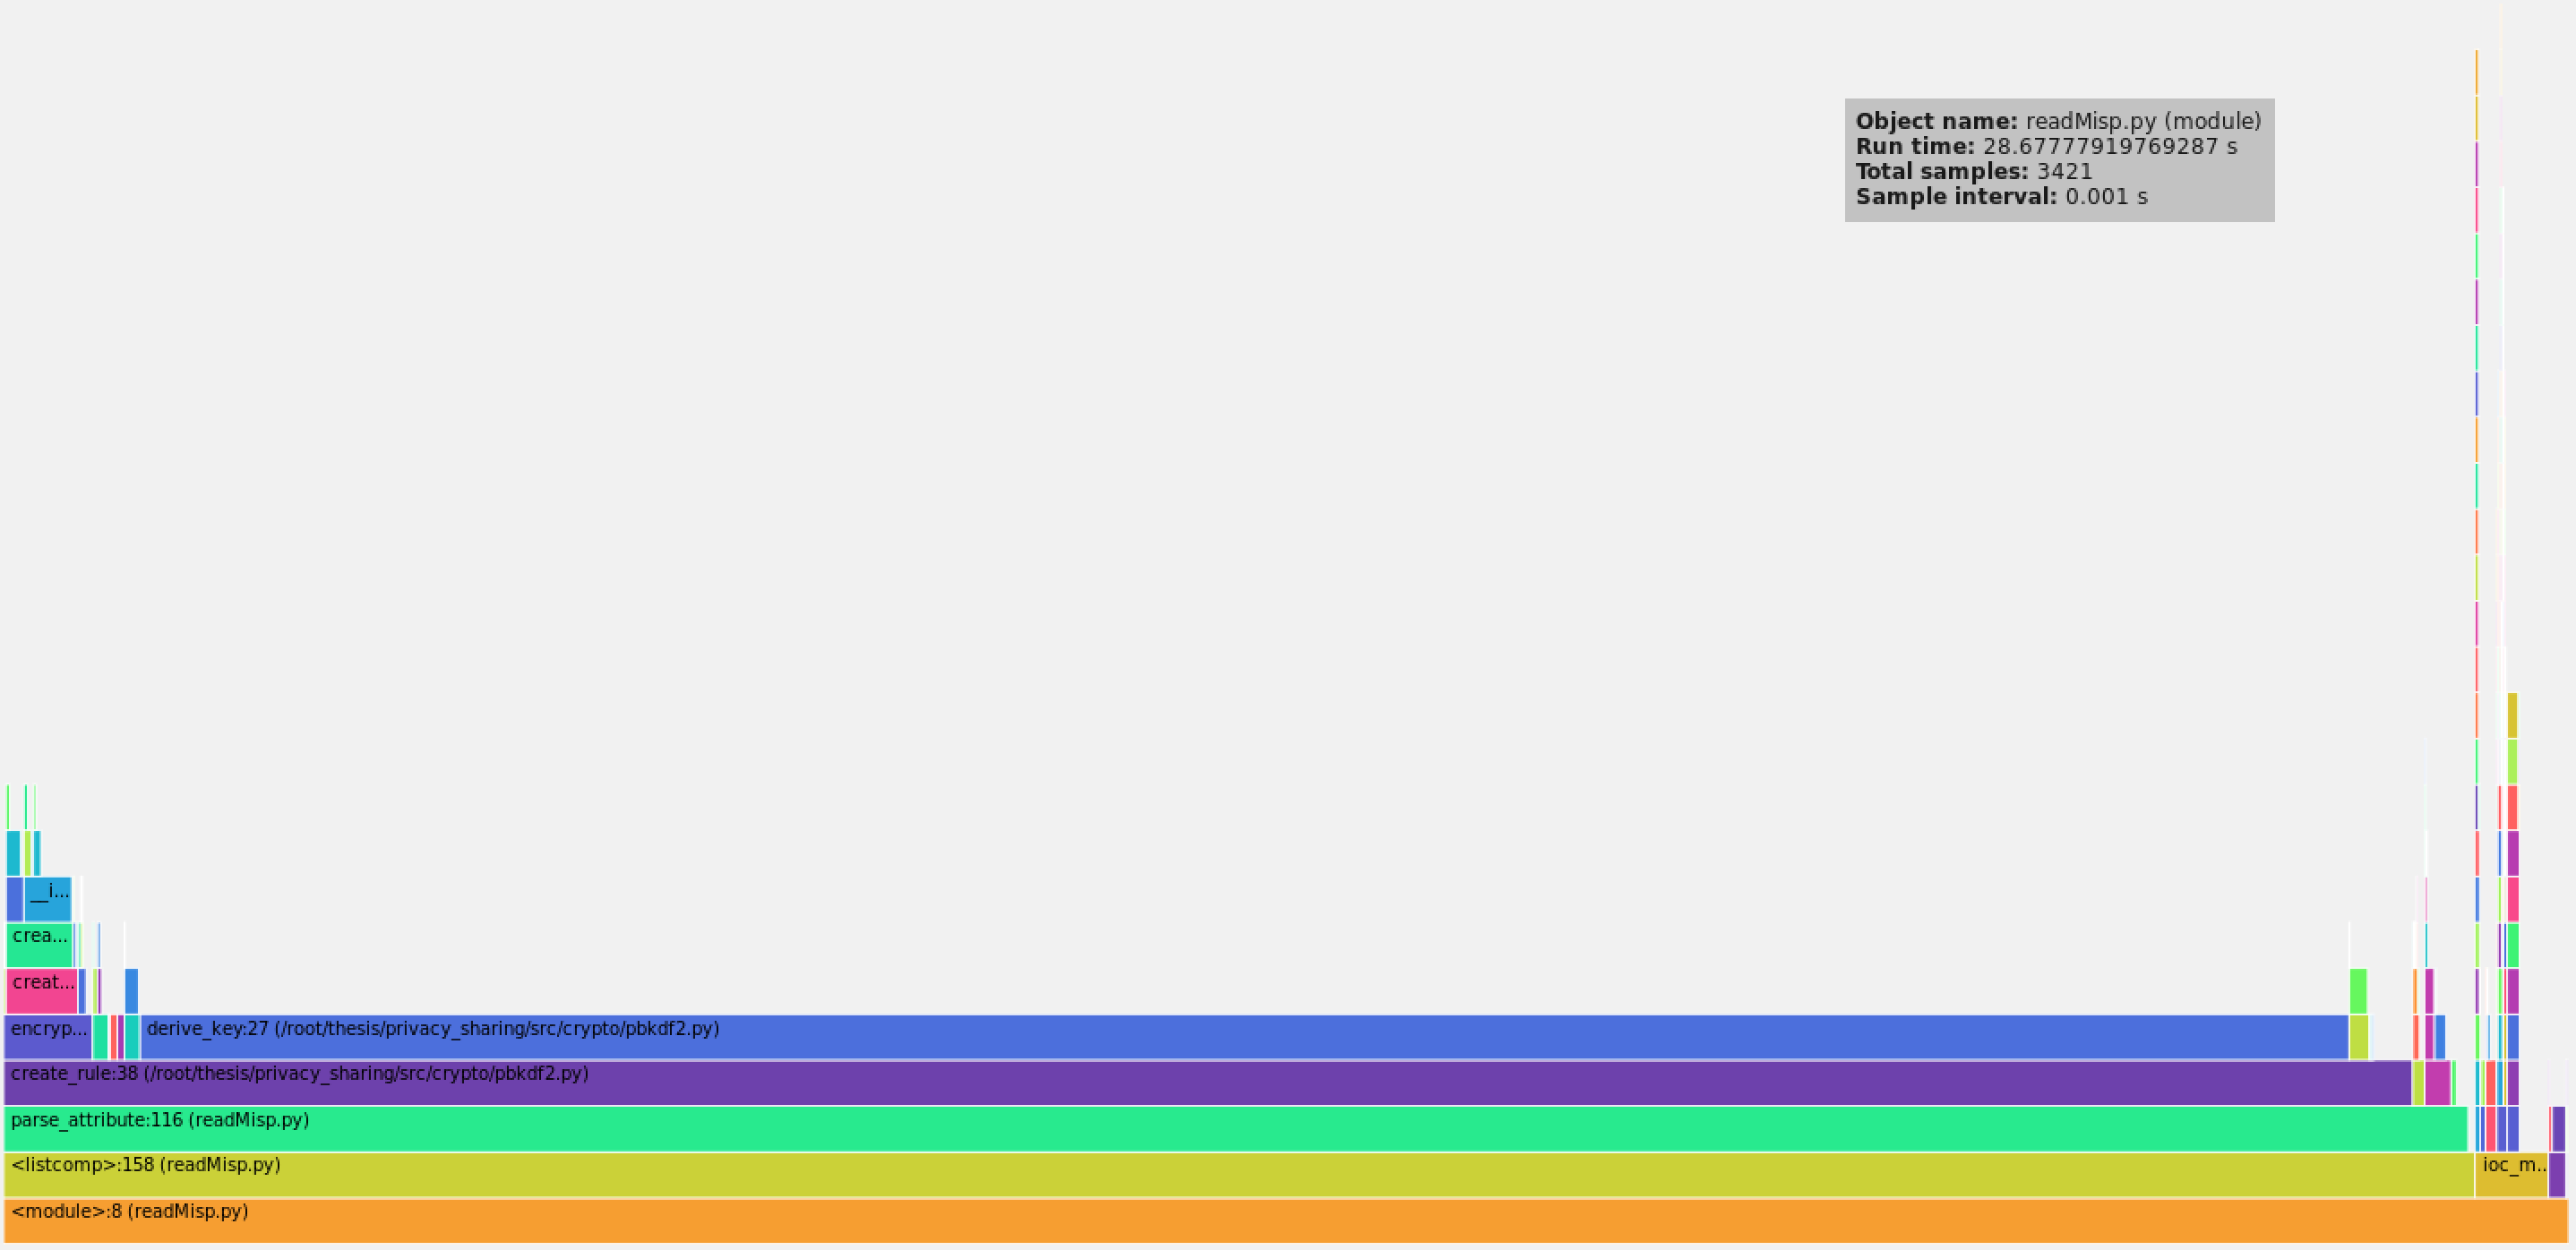
\includegraphics[scale=0.3]{res/profile-1000iter}
	\caption{Vprof - Flame Chart Profile of readMisp PBKDF2(1000 iteration)}
	\label{profile-readMisp1000}
\end{center}
\end{figure}

The goal of this work is to slow down the system, which means that a lot of iteration will be used. \\

\subsection{Profile of the bloomy\_pbkdf2 module}
The first step is to look for the additional computing time for creating the rules and as we can see on figure \ref{}. The key derivation function is still more computationally intensive than the creation of the bloom filter.\\

\improvement{Add picture her but I was not able to do so as my computer is not working anymore}

Then it could be interesting to compare the flow when there is a match and then when the Bloom filter can directly say that the element is not in the set of IOCs.\\

\begin{figure}[h!]
\begin{center}
	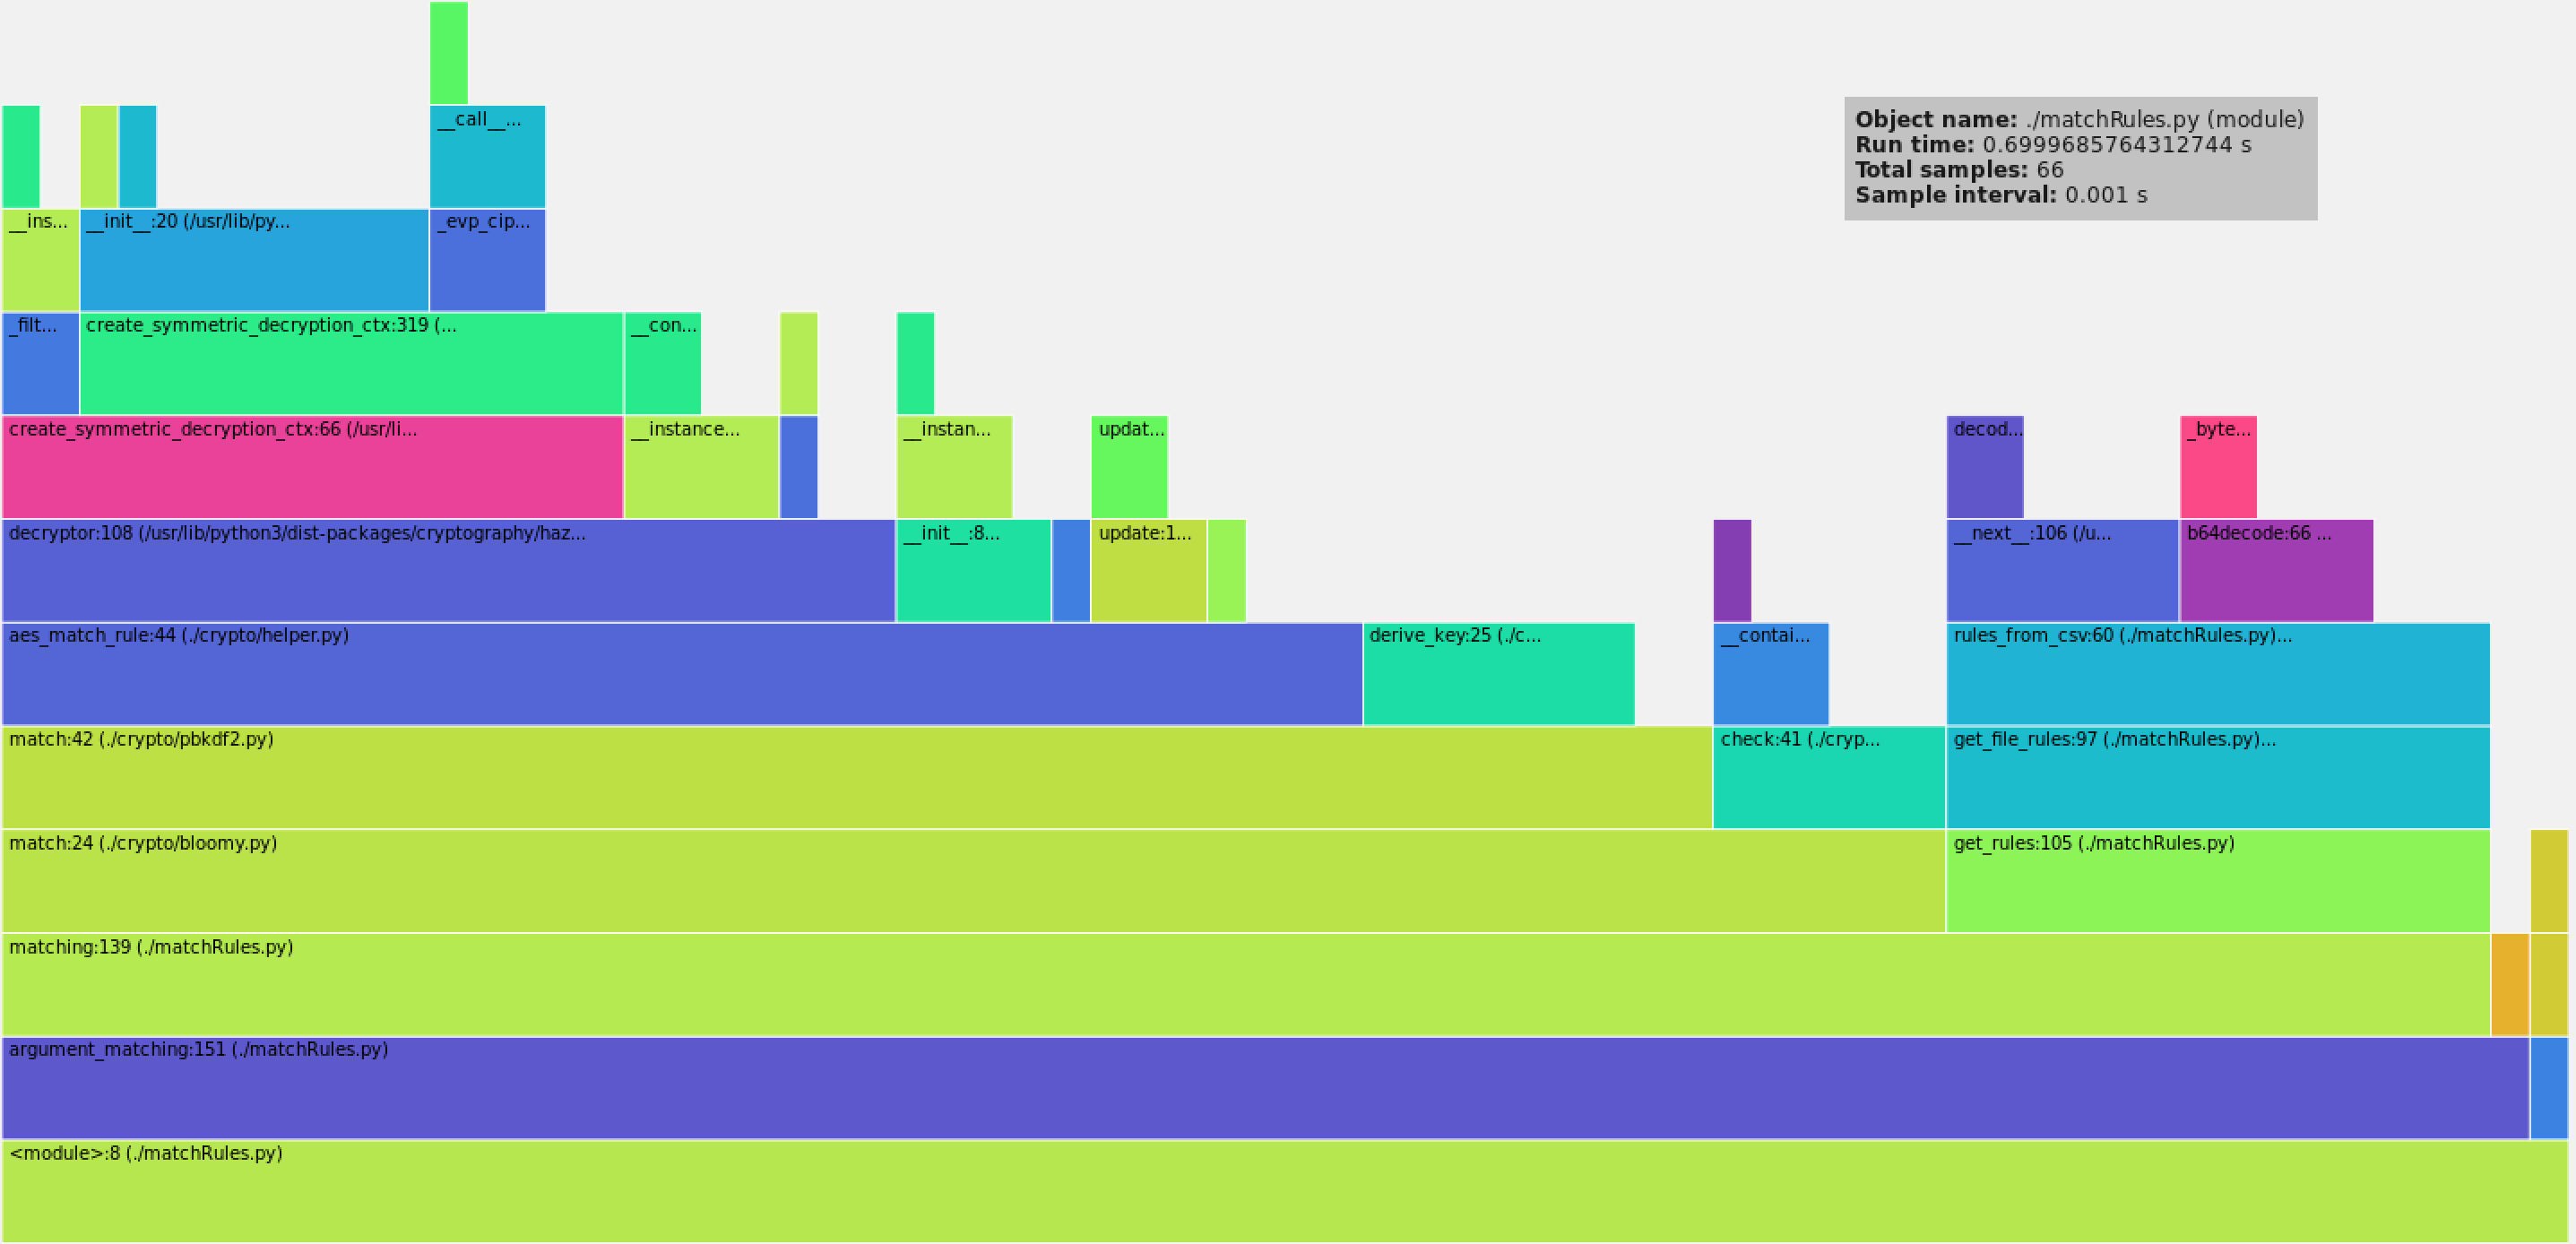
\includegraphics[scale=0.3]{res/match-exist}
	\caption{Vprof - Flame Chart Profile of matchRules bloomy\_pbkdf2 (1 iteration) with a match}
	\label{profile-bloomy-match}
\end{center}
\end{figure}

\begin{figure}[h!]
\begin{center}
	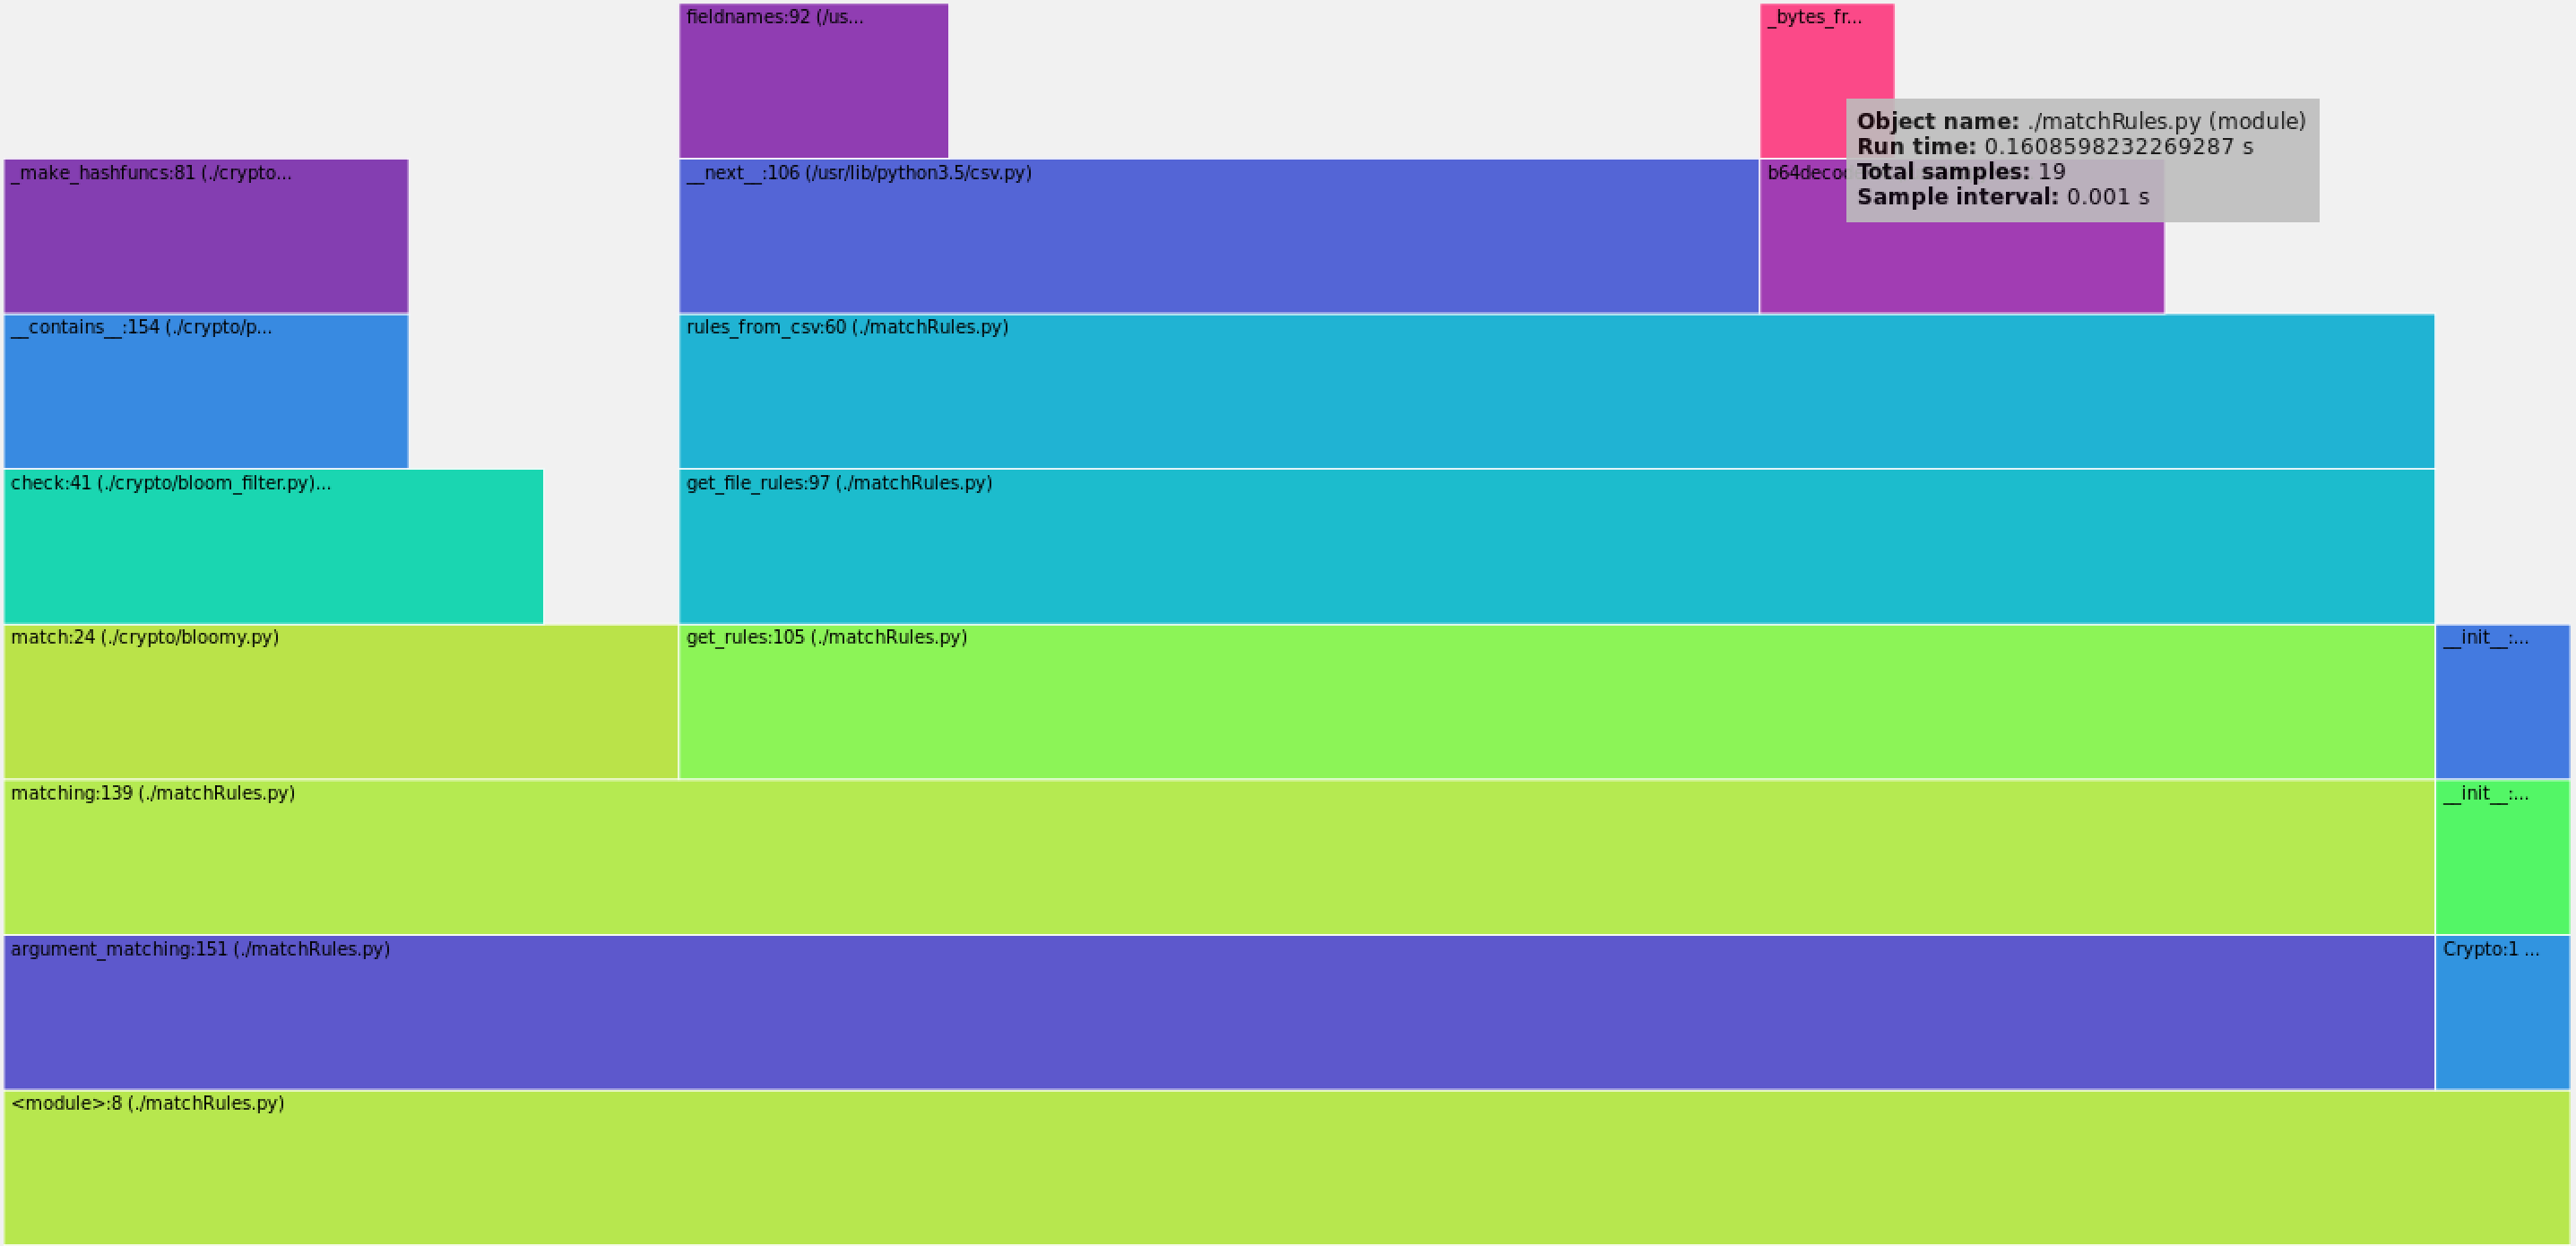
\includegraphics[scale=0.3]{res/match-bloom-not}
	\caption{Vprof - Flame Chart Profile of matchRules bloomy\_pbkdf2 (1 iteration) with no match in the bloom filter}
	\label{profile-bloomy-no-match}
\end{center}
\end{figure}

\section{Benchmarking}
The ideas have been explained, in the first few sections, then the implementation had been explained followed by profiles that help understand how the behavior of the system and how the computation power is used inside the system. Now it is time to see how it is working with real data, what would be the right parameters to use and why these choices. Moreover, this is in this section that we could analyse if the goal had been totally reached, reached for some part and decide if it can or cannot be used in real implementations.\\
This is important as we are aware of the benefits that it could have but we must stay aware of the risk of that exposure on which a system like this one could lead.\\

\improvement{Do all needed analyzes; ajouter brute force de string avec bcrypt => explain expo and why not here}

\section{Security Discussion}
Must be dimensioned carefully !!! => puis expliquer pourquoi c'est trop cool et que l'idée fonctionne vraiment bein mm dans les domaines où on était pas sur

\section{Further Work}
\begin{itemize}
\item Sightings
\item additional crypto systems
\item additional benchmark
\item ...
\end{itemize}


\newpage
\bibliographystyle{acm-doi}
\bibliography{articles}
\newpage

% Back cover page
\backcoverpage




\end{document}
